\documentclass[12pt,oneside]{book}
\usepackage{amsmath}
\usepackage{xcolor}
\setcounter{MaxMatrixCols}{20}

\pagestyle{headings}

% Note that the line below could be modified to suit a
% particular system since the "geometry" package behaves
% differently in Unix, Windows and Mac, especially for the
% top margins.
% Adjust the parameter "top" (measuring the height of the
% space allocated to a header) and "headsep" (measuring
% the distance from the bottom of the header to the
% first line of text.
\usepackage[top=1.3in,left=1.5in,bottom=1in,right=1in,headsep=0.5in]{geometry}

\usepackage{setspace}
\onehalfspacing
%\doublespacing

% Headers and footers for thesis
\usepackage{fancyhdr}

\markboth{}{}
\newcommand\startchapter[1]{\chapter{#1}\thispagestyle{myheadings}}
\newcommand\startappendix[1]{\chapter{#1}\thispagestyle{myheadings}}
\newcommand\startfirstchapter[1]{\chapter{#1}}

% Manual addition of section to Table of Contents
\newcommand\TOCadd[1]{\newpage\phantomsection\addcontentsline{toc}{chapter}{#1}}

% Float Customization
\renewcommand{\floatpagefraction}{0.01}

% Customization of Tables of Contents and List of Figures/Tables
\usepackage{tocloft}
\renewcommand\cfttabpresnum{Table\ }
\renewcommand\cfttabnumwidth{0.75in}
\renewcommand\cftfigpresnum{Figure\ }
\renewcommand\cftfignumwidth{0.80in}
\newcommand{\HRule}{\rule{\linewidth}{0.5mm}}


% Long Table and decimal aligned columns
\usepackage{dcolumn}
\usepackage{longtable}

% Mathematics support
\usepackage{amsmath}
\usepackage{amsthm}
\usepackage{amssymb}
\usepackage{cite}
\usepackage{xfrac}

% Text Control
\usepackage{xspace}
\usepackage{textcase}

% Graphics
\usepackage{wasysym}
\usepackage{graphics}
\usepackage{graphicx}   % A package to allow insertion of
                        % external image files
\usepackage{subcaption}
\usepackage{pbox}



\begin{document}

% Front Matter
\input frontmatter/fm


	\startfirstchapter{Introduction} \label{ch:1}
\section{Background and Motivation}
A surface is what forms a common boundary between two phases of matter. The phases of matter can be of any forms, i.e, solid, liquid, and gas. The behavior of a surface greatly affects the properties of a material, such as oxidation, corrosion, chemical activity, deformation and fracture, surface energy and tension, adhesion, bonding, friction, lubrication, wear and contamination. Therefore, surface characterization identification remains an active area of research in the physics, chemistry, and biotechnology communities as well as in modern electronic technology. It also plays a crucial role in surface science. Among various surface properties, molecular orientation is a key factor of all, because molecular orientation greatly affects molecules' surface properties in aspects such as: adhesion, lubrication, catalysis, bio-membrane functions and so on. \cite{PhysRevB.59.12632}\\

Many experimental techniques have been applied in the study of molecular orientation at surfaces. Among them the optical methods are more preferable. Such methods include infrared (IR) absorption, Raman scattering and visible-infrared sum-frequency generation (SFG) spectroscopies. All these vibrational spectra carry quantitative structural information of molecules at surfaces. Although each of them has its own strengths and shortcomings, they all share the following advantages when compared with other non-optical methods. First of all, they all can be applied to any surfaces accessible by light. Second, they are non-destructive. Third, they offer good spatial, temporal and spectral resolutions \cite{Brasselet:11},\cite{PhysRevB.59.12632}. An important advantage of SFG techniques is that it can discriminate against bulk contributions. This means that its result will not take the effect from the bulk. In order to extract the quantitative structural information that molecules carry at surfaces, different spectroscopy techniques and analysis are required. Combining different spectroscopy techniques is a very effective way to achieve the goal of molecular orientation study at surfaces. However, finding the most effective ways to combine these techniques may not be clear.\\

In order to analyze these vibrational spectra, various factors need to be considered. For example, a molecule's vibrational mode in the molecular frame, the orientation average of the molecules adsorbed onto the surface based on the mathematical orientation distribution function and projecting the vibrational mode properties from molecular frame to laboratory frame. The main focus of my study is combining Linear Programming (LP) with different spectral information to obtain molecular orientation distribution at surfaces. In this thesis, I will explore how LP can facilitate extracting quantitative structural information of molecules at surfaces.\\

My approach is to first study our LP model's properties by applying it to a simplified molecule. After that, the LP model is applied to the representatives of realistic molecules to further explore the possibilities of our LP model. The realistic molecules that I am considering are six amino acids: methionine (Met), leucine (Leu), isoleucine (Ile), alanine (Ala), threonine (Thr) and valine (Val).\\

Before introducing the LP model and the molecule orientation studies, the basic theory of  the IR, Raman and SFG spectra is introduced.\\

\section{Experimental Probes: IR, Raman, SFG Vibrational Spectroscopy}
Vibrational spectra are produced by the changes of a molecule's dipole moment and polarizability. The dipole moment and polarizability are changing as the molecule's conformation is changing. \\

IR is the absorption of passing infrared light through a sample at each frequency, which can be expressed by Equation \ref{eq:1.1}. \\

\begin{equation} \label{eq:1.1}
A_{\rm IR} = - log_{10} \left( \frac{I}{I_{o}} \right)
\end{equation}
where $A_{\rm IR}$ is the measured IR absorbance. $I$ is the light intensity after infrared light pass through the sample. $I_{o}$ is the initial light intensity. \\

The physical principle of IR spectra is the variation of the dipole moment $\mu$ (the first rank tensor) along the normal coordinates $Q$: $\sfrac{\partial\mu}{\partial Q}$. IR spectra can be further expanded by Equation \ref{eq:1.2}.

\begin{equation} \label{eq:1.2}
A_{\rm IR} \approx \left| \frac{1}{\sqrt{2m_{q}w_{q}}} \frac{\partial\mu}{\partial Q} \right|^{2}
\end{equation}
where $m_{q}$ is the reduced mass of the normal mode, and $w_{q}$ is the resonance frequency. The dipole moment $\mu$ is a vector of $x$, $y$ and $z$. The dipole moment derivatives can be expressed as Equation \ref{eq:1.3}. The IR spectra can be obtained from 3 polarizations: $x$, $y$, $z$. \\

\begin{equation} \label{eq:1.3}
\frac{\partial\mu}{\partial Q} = \begin{bmatrix}
									\dfrac{\partial\mu_{x}}{\partial Q} \\
									\dfrac{\partial\mu_{y}}{\partial Q} \\
									\dfrac{\partial\mu_{z}}{\partial Q}
								  \end{bmatrix}
\end{equation}

In the Raman process, stocks-shifted light may be scattered from a molecule sample. Unlike IR, Raman spectra relate to the variation of the molecular polarizability $\alpha$ (the second rank tensor) along the normal coordinates $Q$: $\sfrac{\partial\alpha}{\partial Q}$. \\ 

\begin{equation} \label{eq:1.4}
I_{\rm Raman} \approx \left| \frac{1}{\sqrt{2m_{q}w_{q}}} \frac{\partial\alpha^{(1)}}{\partial Q} \right|^{2}
\end{equation}
where $m_{q}$ and $w_{q}$ are the same as defined in Equation \ref{eq:1.2}. The polarizability is coupled with $x$, $y$, $z$ components of the driving field and $x$, $y$, $z$ components of the induced polarization. Therefore, there are 9 elements in the polarizability, which can be expressed as Equation \ref{eq:1.5}. It results in 9 polarizations of Raman spectra: $xx$, $yy$, $zz$, $xy$, $xz$, $yx$, $yz$, $zy$ and $zx$. \\

\begin{equation} \label{eq:1.5}
\frac{\partial\alpha^{(1)}}{\partial Q} = \begin{bmatrix}
\dfrac{\partial\alpha_{xx}^{(1)}}{\partial Q} & \dfrac{\partial\alpha_{xy}^{(1)}}{\partial Q} & \dfrac{\partial\alpha_{xz}^{(1)}}{\partial Q} \\
\dfrac{\partial\mu_{yx}}{\partial Q} & \dfrac{\partial\alpha_{yy}^{(1)}}{\partial Q} & \dfrac{\partial\alpha_{yz}^{(1)}}{\partial Q}\\
\dfrac{\partial\mu_{zx}}{\partial Q} & \dfrac{\partial\alpha_{zy}^{(1)}}{\partial Q} & \dfrac{\partial\alpha_{zz}^{(1)}}{\partial Q}
\end{bmatrix}
\end{equation}

SFG stands for sum frequency generation vibrational spectroscopy. SFG is a surface-specific technique. It is a non-linear optical process. SFG is the variation of the outer product of dipole moment and polarizability, $\alpha^{(2)}$ (the third rank tensor): $\frac{\partial\mu}{\partial Q} \otimes \frac{\partial\alpha}{\partial Q} $. Therefore, there are 27 elements for SFG spectra, which result in 3 unique polarizations of SFG spectra: $xxz$, $xzx$, and $zzz$. \\

\begin{equation} \label{eq:1.6}
I_{\rm SFG} \approx \left| \alpha^{(2)}_{ijk} \right|^{2}
= \left| \frac{1}{2m_{Q}w_{Q}} \left( \frac{\partial\alpha^{(2)}_{ij}}{\partial Q} \otimes \frac{\partial\mu_{k}}{\partial Q} \right) \right|^{2}
\end{equation}

\section{Linear Programming}
LP problems are optimization ones of a specific form. The standard form of LP is a minimization problem that has an objective function and a number of constraints as shown in Equation \ref{eq:1.7} \cite{UULP}:

\begin{eqnarray}  \label{eq:1.7}
 \text{minimize} & c_{1}x_{1} + c_{2}x_{2} + ... + c_{n} x_{n}  \nonumber \\
 \text{subject to} & a_{11} x_{1} + a_{12} x_{2}+ ... + a_{1n} x_{n} = & b_{1} \nonumber \\
& a_{21} x_{1} + a_{22} x_{2} + ... + a_{2n} x_{n} = & b_{2} \nonumber \\
&\vdots                                   &\vdots \nonumber \\
& a_{m1} x_{1} + a_{m2} x_{2} + ... + a_{mn} x_{n} = & b_{m} \nonumber \\
& x_{1} \geq 0, x_{2} \geq 0, ... ,x_{n} \geq 0, 
\end{eqnarray} 
where $x_{i}$ are the decision variables, $a_{ij}$ is a matrix of known coefficients, $b_{i}$ and $c_{i}$ are vectors of known coefficients. The expression to be minimized is called objective function. The equalities and the inequalities are the constraints that all the decision variables need to subject to. These constraints specify a convex polytope that the objective function need to optimize over. \\ 

The diet problem is a popular example to illustrate the concept of LP. It is described as follows: a restaurant would like to achieve the minimal nutrition requirements with the lowest price over some food selections as shown in Table \ref{tab:1.1}. For each meal, the minimum requirements for vitamin A, vitamin C and dietary fiber are $0.5 \rm mg$, $15 \rm mg$ and $4 \rm g$. The restaurant has three food options: raw carrot, raw white cabbage and pickled cucumber. The table also displays the nutrition content and the price of each ingredient. With all the information, we want to know how much carrot, cabbage and cucumber is needed in each meal, so that the minimal nutrition requirements can be met with the lowest price. In summary, the goal is to minimize the price, and the constraints are the nutrition requirements. Therefore, the following LP model is formulated as shown in Equations from \ref{eq:1.8} to \ref{eq:1.14}.

\begin{table} 
\begin{center}
\begin{tabular}{| l | l  l  l | l |}
\hline
Food & Carrot & Cabbage & Cucumber & Required per dish \\ \hline
Vitamin A [mg/kg] & 35 & 0.5 & 0.5 & 0.5mg \\ 
Vitamin C [mg/kg] & 60 & 300 & 10 & 15mg \\ 
Dietary Fiber [g/kg] & 30 & 20 & 10 & 4g \\ \hline
price[$\$$/kg] & 0.75 & 0.5 & 0.15 & - \\ \hline
\end{tabular} 
\end{center}
\caption{Sample input of the diet problem}
\label{tab:1.1}
\end{table}	

\begin{eqnarray} 
\text{minimize} & 0.75x_{1} + 0.5x_{2} +  0.15x_{3}  \label{eq:1.8} \\
\text{subject to} & 35x_{1} + 0.5x_{2} + 0.5x_{3} \geq 0.5 \label{eq:1.9} \\
& 60x_{1} + 300x_{2} + 10x_{3} \geq 15 \label{eq:1.10} \\
& 30x_{1} + 20x_{2} + 10x_{3} \geq 4 \label{eq:1.11} \\
& x_{1} \geq 0  \label{eq:1.12} \\
& x_{2} \geq 0  \label{eq:1.13} \\
& x_{3} \geq 0  \label{eq:1.14}
\end{eqnarray} 
where $x_{1}$, $x_{2}$ and $x_{3}$ are the decision variables. Each decision variable presents the amount of each ingredient. Equation \ref{eq:1.8} is the objective function to minimize. Equation \ref{eq:1.9} to Equation \ref{eq:1.11} describe the nutrition requirements. Equation \ref{eq:1.12} to Equation \ref{eq:1.14} ensure the amount of each ingredient to be greater than 0. The coefficients in the objective function represent $c_{i}$ vector in Equation \ref{eq:1.1}. The coefficients of the decision variables in Equation \ref{eq:1.9}, \ref{eq:1.10} and \ref{eq:1.11} represent $a_{ij}$ matrix. $b_{i}$ vector is composed by the right-hand side of Equation \ref{eq:1.9}, \ref{eq:1.10} and \ref{eq:1.11}. \\

In order to apply simplex method, the above LP problem needs to transfer into its standard form. The inequalities of Equations from \ref{eq:1.9} to \ref{eq:1.11} need to transform to equalities. Therefore, a new variable, called a slack variable (SV) is introduced to change each inequality to equality \cite{ConvexOptimization}. \\

With the existing LP solvers that implemented simplex method, the optimal solution can be obtained within a second. \\

For a LP problem, there are only three kinds of solutions: feasible and bounded, feasible and unbounded, and infeasible. If the solution space is feasible and bounded, then there is one optimum solution. If it is feasible but unbounded, then there is a solution space with an infinite number of optimal solutions \cite{LP}. \\

A general LP problem can be a minimization or maximization problem. Its constraints can be equalities or inequalities. For each non-standard LP problem, there are ways to convert it into its standard form. Furthermore, for a LP problem that contains $n$ decision variables, its solution would be in a $n$-dimensional space called $R^{n}$. Each constraint is a hyperplane. It divides the $R^{n}$ space into two half-spaces. Therefore, all the constraints together cut this $R^{n}$ space into a convex polyhedron when there are feasible solutions. This makes LP a convex problem. The benefit of a convex problem is that the local optimal solution is the global optimum. LP solvers return the optimal solution. If a LP problem has a unique optimal solution, this solution is a vertex of the convex polyhedron. In other words, LP is a convex, deterministic process. It is guaranteed to converge to a single global optimum if there is a bounded solution space. \\

Another advantage of LP is that it can deal with tens or hundreds of thousands of variables, which makes it suitable for the study of a molecule's orientation distribution at surfaces. Furthermore, LP problems are intrinsically easier to solve than many non-linear problems. \\

Various algorithms are available in solving LP problems, such as: simplex algorithm, interior point, and path-following algorithms. Both interior point and simplex are common and mature algorithms that work well in practice. Simplex is comparatively easier to understand and implement than interior point. Simplex method takes the advantage of the geometric concept that it visits the vertices of the feasible set (convex polyhedron), and checks the optimal solution among each visited vertex. The converging approach is different for these two methods. If there are $n$ decision variables, usually simplex method converges in $O(n)$ operations with $O(n)$ pivots. Interior point traverses the edges between vertices on a polyhedral set. Generally speaking, Interior point method is faster for larger problems with sparse matrix. However, when experimenting with these two methods, the speed of them is not much different from each other for my study. In my study, simplex method has proved to be efficient and effective, and it is used for all the test cases. \\

Last but not the least advantage of LP is its speed. For any LP problem, if it has an optimal solution, this solution is always a vertex. Simplex method is based on this insight, namely that it starts at a vertex, then pivot from vertex to vertex, until it reaches the optimum. Although it has been shown that simplex method is not a polynomial algorithm, in practice it usually takes $2n\sim3n$ steps to solve a problem ($n$ is the number of the decision variables). Currently there are two main approaches in studying the orientation distribution of molecules at surface. One is comparing the experimental spectra with few predicted ones, and select the one that most matches to the experimental one. Another one is running an exhaustive algorithm to explore the most possible solution space \cite{hore0033-rotations}. However, both approaches take a lot of time and computational resources. Therefore, applying LP will result a large gain in computation.\\

The LP solver we use is called ``GNU linear programming tool kit" (GLPK). It has implemented both simplex and interior point methods in C programming language. It is open-source and intended to solve large scale LP problems. \\

\section{Conclusion and Open Questions from Previous Study}
%In Hung's study \cite{KuoKaiHung:Thesis:2015}, the new approach of applying LP to vibrational spectra to extract the molecular orientation distribution at surfaces is introduced. The LP approach helped to return the target orientation distribution information when the mock experimental spectrum consisted of different amino acids. However, when candidates are coming from the same amino acid, LP approach failed to return the target orientation distribution information. The reason why LP failed to return the target composition has not been thoroughly studied in Hung's study. Whether and how LP approach can be generally applied to different case studies have not been explored neither. Moreover, in Hung's study, only SFG spectral information is applied to the LP model. The case of combining different spectral techniques to the LP model was not considered. Only mock experimental spectral information is considered.

My research is based on Hung's study \cite{KuoKaiHung:Thesis:2015}. In his study, he mentioned that generating model spectra that match the target experimental spectra from a list of known candidates is a way to extract molecular orientation information at surface. The traditionally exhaustive way of achieving this goal consumes too much computational effort, therefore, he introduced LP approach to vibrational spectroscopy study. The LP approach results in pseudo polynomial time $O(n)$, which is a great improvement compared to $O(n!)$. \\

However, depends on different test case settings, the LP approach may not always return the target composition of candidates that generates the mock target experimental spectra. When considering the candidates from one type of molecule at surfaces, the return solution of the LP approach does not match the known target composition. When considering the candidates from a mixture of molecules, the return solution of the LP approach does match the know target composition. The reason why the LP approach failed to return the target composition has not been thoroughly studied by Hung. \\

Moreover, when applying the LP approach, only SFG spectral information has been considered in his LP model. The possibility and applicability of using IR and Raman spectral information to the LP approach have not been considered. Meanwhile, the possibility of combining different spectral information to the LP approach has not been considered neither. \\
	
\section{Aims and Scope}
The goal of my study is to figure out the underlying properties of the LP approach, figure out what is the cause that the LP approach fails to obtain the target composition of candidates in some test cases. Based on the gained information, I further explore the applicability of the LP approach to different test cases. My plan is applying the LP approach to a simplified molecular model first, so that only the properties of our LP model can be focused. \\

With the properties learnt from the first step, the LP approach is then applied to realistic molecules. There are two types of test cases, one is considering the candidates coming from one type of realistic molecule, to see if the LP approach can return the target composition of the mock spectra. Another one is considering the candidates coming from different types of realistic molecules. If the LP approach achieve in obtaining the target composition, then how the LP approach applied systematically will be studied. \\

The purpose is to check if LP approach will return the target composition of the spectra for one type of molecule at surfaces. If yes, whether the LP model can be applied generally to one type molecule will be studied. If not, what is the underlie reason will be explored. Similar study will also be applied to different molecules at surfaces. At last, the experimental spectral information is brought into consideration. \\

\section{Overview of the Thesis}
Chapter \ref{ch:1} briefly introduces the aim and scope of the current study. Chapter \ref{ch:2} explains the current approaches to extract the molecular orientation distribution at surfaces, as well as how to produce IR, Raman and SFG spectra. Chapter \ref{ch:3} aims to use a simplified molecular model to study the properties of our LP model. Chapter \ref{ch:4} applies our LP approach to one type of molecule at surfaces. Chapter \ref{ch:5} applies the LP approach to a mixture of different molecules at surfaces. Chapter \ref{ch:6} applies the LP approach to experimental spectral data. Chapter \ref{ch:7} is the conclusion and future work.

	\startchapter{Methods} \label{ch:2}
\section{Description}
Before introducing and analyzing the LP model and applying it to the realistic molecules' vibrational spectra, there are a few factors to address. First of all, creating each amino acid's IR, Raman and SFG spectra is an essential step. This part research has been done thoroughly by Hung \cite{KuoKaiHung:Thesis:2015}. In this chapter, I introduce the content that is related to our study. \\

\section{Structure of Realistic Molecules}
Figure \ref{fig:aminacids} illustrates the molecule structure of the six amino acids in the molecular frame. These amino acids are used in the test cases related to realistic molecules. The $a$, $b$ and $c$ are the molecular frame coordinates. When a molecule lays on a surface, we need to transfer the molecular frame to the lab frame where the surface exists. \\

\begin{figure}
\begin{subfigure}{.5\textwidth}
  \centering
  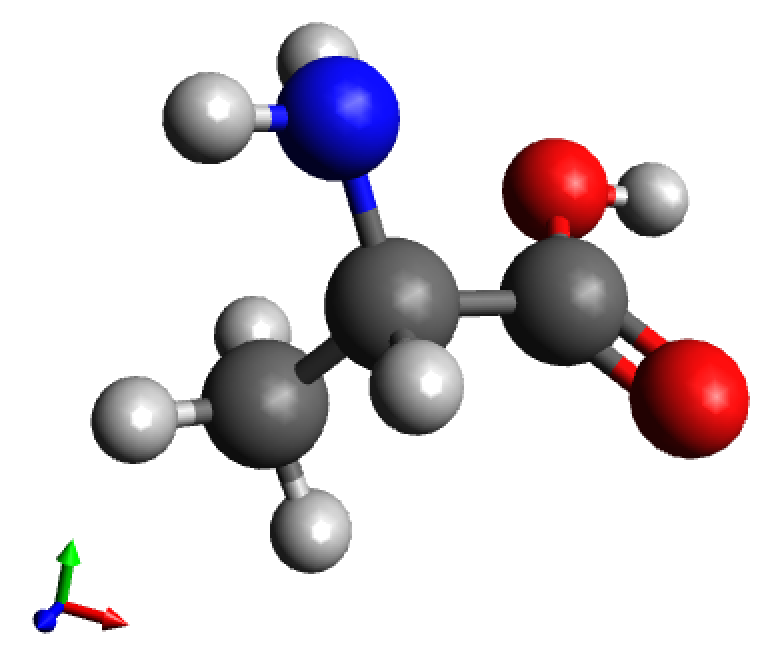
\includegraphics[height=5cm]{Figures/Ala.png}
  \caption{Ala}
  \label{fig:sfig1}
\end{subfigure}%
\begin{subfigure}{.5\textwidth}
  \centering
  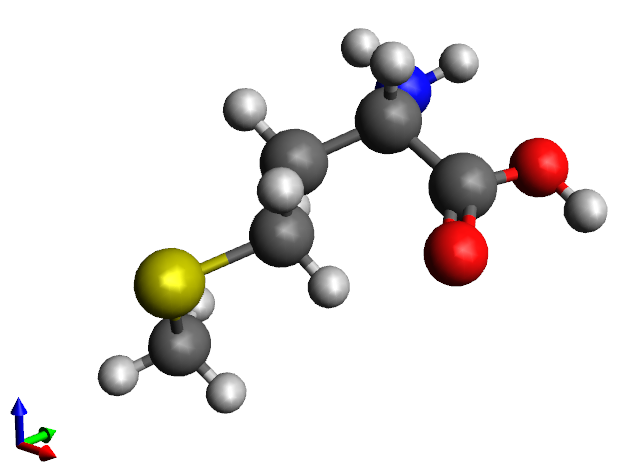
\includegraphics[height=5cm]{Figures/Met.png}
  \caption{Met}
  \label{fig:sfig2}
\end{subfigure}
\begin{subfigure}{.5\textwidth}
  \centering
  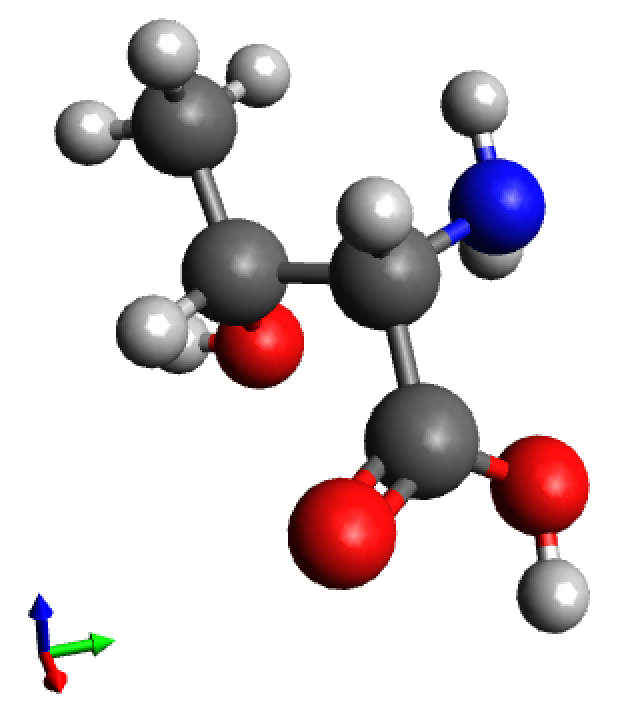
\includegraphics[height=5cm]{Figures/Thr.png}
  \caption{Thr}
  \label{fig:sfig3}
\end{subfigure}
\begin{subfigure}{.5\textwidth}
  \centering
  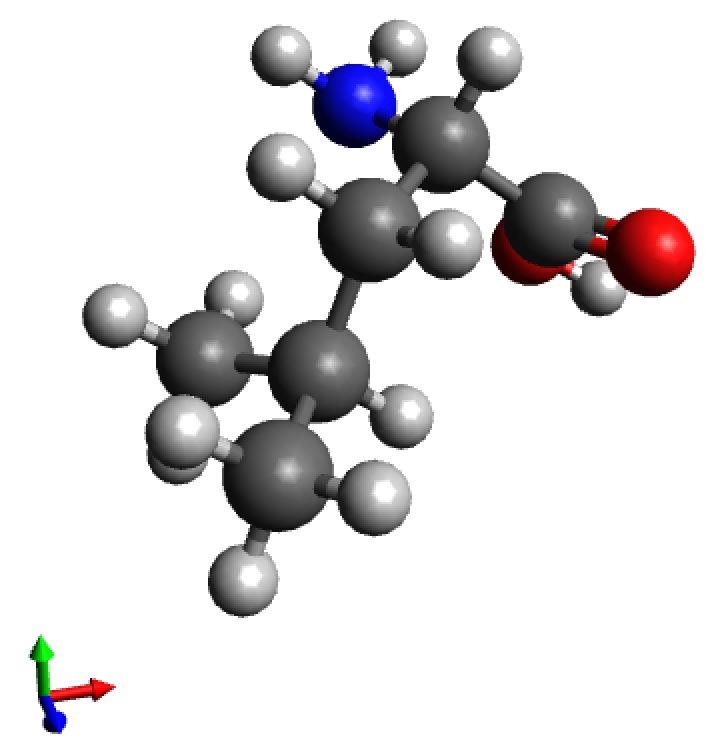
\includegraphics[height=5cm]{Figures/Leu.png}
  \caption{Leu}
  \label{fig:sfig4}
\end{subfigure}
\begin{subfigure}{.5\textwidth}
  \centering
  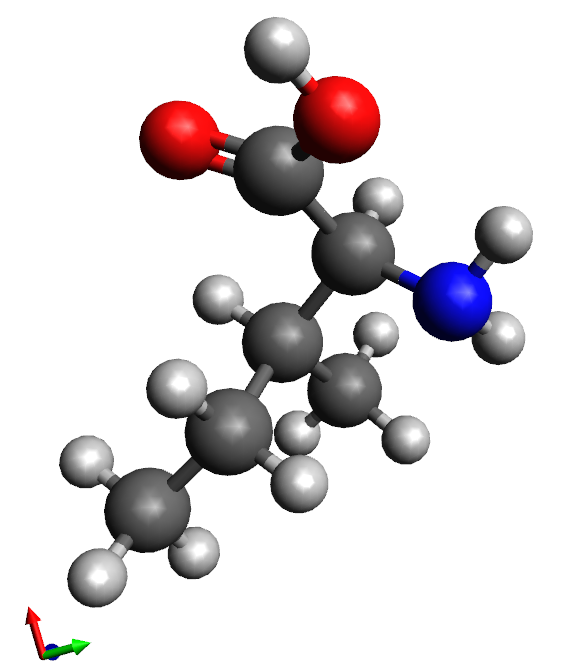
\includegraphics[height=5cm]{Figures/Ile.png}
  \caption{Ile}
  \label{fig:sfig5}
\end{subfigure}
\begin{subfigure}{.5\textwidth}
  \centering
  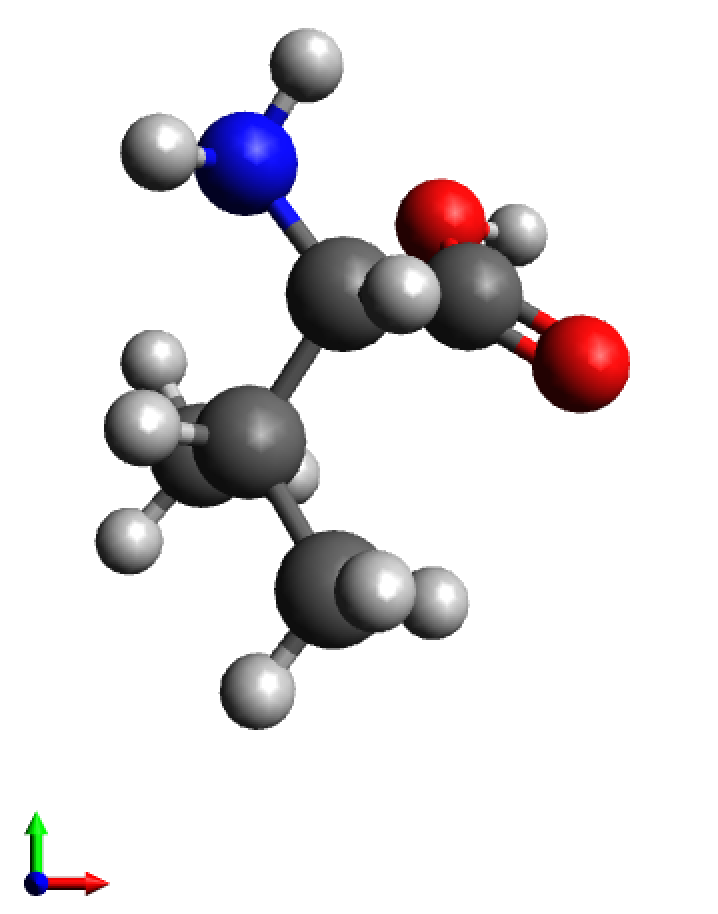
\includegraphics[height=5cm]{Figures/Val.png}
  \caption{Val}
  \label{fig:sfig6}
\end{subfigure}
\caption{Molecule structure of Ala, Met, Thr, Leu, Ile and Val in molecular frame. Blue axis is designated as $c$ axis, red axis is designated as $a$ axis, green is designated as $b$ axis. The blue atoms are Nitrogen, the red atoms are Oxygen, the black atoms are Carbon, the while atoms are Hydrogen.}
\label{fig:aminacids}
\end{figure}

\section{Generating Model Spectra \cite{ss}}
To generate these amino acids' vibrational spectra, a molecule's vibration modes need to be modelled in the molecular frame, and then transferred to the laboratory frame where surfaces exist. Chapter 2 in Hung's thesis \cite{KuoKaiHung:Thesis:2015} describes how to perform electronic structure calculations using a software package called The General Atomic and Molecular Electronic Structure System (GAMESS) \cite{GAMESS} to obtain the derivatives of every dipole moment and polarizability. Then he introduced how to use Direction Cosine Matrix (DCM) to transfer these two derivatives from the molecular frame to the laboratory one. After that, Euler angles could be extracted from DCM. Euler angles are used to describe a molecule's orientation at surfaces. They are labelled by $\theta$, $\varphi$ and $\psi$ as shown in Figure \ref{fig:2.1}. They are referred to as $tilt$, $azimuthal$ and $twist$ angles, respectively. Let $x$, $y$ and $z$ be lab frame Cartesian coordinates, and let $a$, $b$ and $c$ be the molecular frame coordinates. $Tilt$ angle $\theta$ is the angle between $z$ and $c$. $Azimuthal$ angle $\varphi$ is the rotation about $z$. $Twist$ angle $\psi$ is a twist about $c$ \cite{hore0033-rotations}. After three steps of successive rotations of Euler angles, molecule properties can be transferred from the molecular frame to the lab one. \\

In order to achieve the above steps, Hung first did a Hessian calculation using GAMESS. Secondly, seven snapshots of a molecule vibrating in different modes were taken. Thirdly, he did a force field calculation to obtain the derivatives of dipole moment and polarizability for each of the seven snapshot moment. Then the derivatives of dipole moment and polarizability are obtained by the interpolation of these seven snapshot moment. Because the two obtained derivatives are in the molecular frame, Hung used DCM to convert these two derivatives into the lab frame. Then he abstracted Euler angles from DCM. After these electronic structure calculations, the derivatives information, which is the molecular property information, is obtained. \\

\begin{figure}[!ht] 
\centering
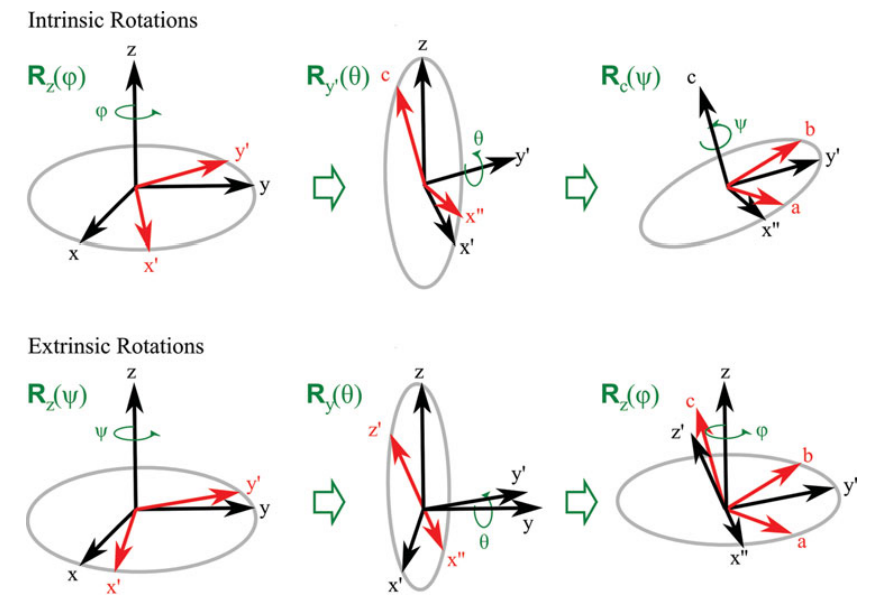
\includegraphics[scale=0.5]{Figures/Euler_angles_represented_as_the_spherical_polar_angles.png} 
\caption{The Euler angles represented as the spherical polar angles $\theta$, $\varphi$ and $\psi$, and the illustration of the three successive rotations that transform the lab $x$, $y$, $z$ coordinate system into the molecular $a$, $b$, $c$ frame intrinsically and extrinsically. Reproduced from Ref. \citenum{hore0033-rotations}. }
\label{fig:2.1}
\end{figure}

In our study, those molecular property information is used to generate the amino acids' spectral information directly. Each molecule's property information contains the derivatives of dipole moment and polarizabilities of each vibrational mode. Depending on the number $N$ of atoms in a molecule, there are $3N-6$ vibrational modes. Furthermore, Equations \ref{eq:2.2} to \ref{eq:2.4} are used to generate the amino acids' IR, Raman and SFG spectra. \\

All the test cases in our study are limited to only consider the $tilt$ angle distribution of Euler angles, and assume isotropy on $twist$ and $azimuthal$ angular distributions. A uniform distribution is applied to $twist$ and $azimuthal$ angles. For angle $\varphi$, it requires the surfaces to be not striped, which means the surface does not have any pattern. Therefore, the molecule has no preference on the $xy$ plane on the lab frame. There can be no anisotropy in the plane of the surface. Because of this, we can limit the candidate number by integrating angle $\varphi$. For angle $\psi$, a uniform distribution implies that a molecule has cylindrical symmetry in its preference of surface. The molecule can be tilted, but has no `$twist$' preference. With the integration of these two Euler angles, the number of candidates for one molecule will be greatly reduced. Therefore, a candidate in our study is a specific molecule with specific $\theta$ value. However, the number of the candidates is still large when considering angle $\theta$ only. For example, from $0^{\circ}$ till $180^{\circ}$, candidates are obtained in $10^{\circ}$ steps, there are $18$ candidates for just one molecule. For a mixture of six molecules, the number of possible combinations of all these molecules' candidates is $18^{6} = 34012224$. \\

When molecules lay on a surface, the orientation of each single molecule varies. To simulate the vibrational spectra, a reasonable orientation distribution for the molecules needed to be studied. The orientation distribution requires either to do a molecular dynamic simulation in order to study the distribution of molecule orientations at surface, or come up with an analytic orientation distribution function. In our study, the LP approach is appropriate for the second method. Moreover, the $\delta$-distribution function shown in Equation \ref{eq:2.1} is used to represent the molecule orientation distribution that models the spectrum signals. This means that all the molecules are tilted at the same angle at surface. This assumption is applied across the whole study. \\

\begin{equation} \label{eq:2.1}
f_{(\theta)} = \delta(\theta - \theta_{o})
\end{equation} 

The absorption of an IR spectrum is proportional to the square of the lab-frame dipole moment derivative. For example, the $x$-polarized absorption spectrum is given by Equation \ref{eq:2.2}: \\

\begin{equation} \label{eq:2.2}
A_x(\omega_{\rm IR}) = \sum_{q} \frac{1}{2 m_{q} \omega_{\rm q}} \Bigg \langle \Bigg\lbrack \frac{\partial u_x}{\partial Q} \Bigg\rbrack_{q} ^2 \Bigg\rangle \frac{\Gamma_q^2}{(\omega_{\rm IR}-\omega_{\rm q})^2 + \Gamma_q^2}
\end{equation} 
where $A_x$ represents $x$-polarized IR obsorbance. $\omega_{\rm IR}$ is the frequency of the probe radiation, $\mu$ is the dipole moment, $m_q$ is the reduced mass, $w_q$ is resonance frequency. $\Gamma_q$ is the homogeneous line width, is set to $6$ in all the test cases. $Q_q$ is the normal mode coordinate of the $q$th vibrational mode. All values of $\omega_{\rm IR}$, $\mu$, $m_q$, $Q$ are obtained from the electronic structure calculations. Furthermore, because $\varphi$ and $\psi$ angles are assumed to be isotropic, the $x$-polarized spectrum is identical with the $y$-polarized one. Therefore, there are only two unique polarized IR spectra. For simplicity, IR spectra are referred to as $x$ and $z$ in future test cases. $A_y$ and $A_z$ are computed accordingly.\\

The intensity of Raman scattering is proportional to the square of lab frame transition polarizability. For example, Raman spectroscopy with an $x$-polarized excitation source collects the $x$-polarized component of the scattered radiation, which can be approximated using Equation \ref{eq:2.3}. \\

\begin{equation} \label{eq:2.3}
I_{xx}(\Delta \omega) = \sum_{q} \frac{1}{2 m_{q} \omega_{\rm q}} \Bigg \langle \Bigg\lbrack \frac{\partial \alpha_{xx}^{(1)}}{\partial Q} \Bigg\rbrack_{q} ^2 \Bigg\rangle \frac{\Gamma_q^2}{(\Delta \omega-\omega_{\rm q})^2 + \Gamma_q^2}
\end{equation} 
where $I_{xx}$ represents $xx$-polarized Raman intensity. $\Delta w$ is the Stokes Raman shift. $\alpha_{xx}^{(1)}$ is one component of the nine-element polarizability tensor. $m_q$, $w_q$, $\Gamma_q$, and $Q_q$ are the same as defined above for IR spectra. All the values of $\omega_{\rm IR}$, $\mu$, $m_q$, $Q$ are obtained from the electronic structure calculations. Similar to IR spectroscopy, because of the integration of $\varphi$ and $\psi$ angles, only four unique spectra are obtained from the following polarization: $xx$, $xy$, $xz$ and $zz$. For simplicity, Raman spectra are referred to as $xx$, $xy$, $xz$ and $zz$ in future test cases. \\

%The intensity of SFG spectroscopy is proportional to the squared magnitude of the second-order susceptibility, $\left|\chi^{(2)}\right|^{2}$. $\chi^{(2)}$ is derived from the second-order polarizability, $\alpha^{2}$. 
SFG spectral signal is the imaginary part of the second-order susceptibility, $\left|\chi^{(2)}\right|$. $\chi^{(2)}$ is derived from the second-order polarizability $\alpha^{(2)}$ as shown in Equation \ref{eq:kai}. The imaginary part of $\left|\chi^{(2)}\right|$, which is the SFG spectral signal, is displayed as Equation \ref{eq:2.4}.

\begin{equation} \label{eq:kai}
\chi^{(2)}_{xxz} (\omega_{\rm IR}) = \sum_{q} \frac{1}{2 m_{q} \omega_{\rm q}} \Bigg \langle \Bigg\lbrack \frac{\partial \alpha_{xx}^{(1)}}{\partial Q} \Bigg\rbrack_{q} \Bigg\lbrack \frac{\partial u_{z}}{\partial Q} \Bigg\rbrack_{q} \Bigg\rangle \frac{1}{\omega_{\rm q}-\omega_{\rm IR}+i\Gamma_q}
\end{equation} 

\begin{equation} \label{eq:2.4}
\rm Im \Bigg\lbrack \chi^{(2)}_{xxz} (\omega_{\rm IR}) \Bigg\rbrack= \sum_{q} \frac{1}{2 m_{q} \omega_{\rm q}} \Bigg \langle \Bigg\lbrack \frac{\partial \alpha_{xx}^{(1)}}{\partial Q} \Bigg\rbrack_{q} \Bigg\lbrack \frac{\partial u_{z}}{\partial Q} \Bigg\rbrack_{q} \Bigg\rangle \frac{\Gamma_q}{(\omega_{\rm q}-\omega_{\rm IR})^{2}+\Gamma_q^{2}}
\end{equation} 
where $\chi^{(2)}_{xxz}$ is the second-order susceptibility. It is probed by an $x$-polarized visible incoming beam at frequency $\omega_{\rm vis}$ and a $z$-polarized infrared beam incoming with frequency $\omega_{\rm IR}$. Both incoming beams are incident to the sample. Then the $x$-component at frequency $\omega_{\rm SFG}=\omega_{\rm vis}+\omega_{\rm IR}$ is selected for detection. As $i=\sqrt{-1}$ is in the denominator, $\chi^{(2)}$ is a complex value \cite{KuoKaiHung:Thesis:2015}. The SFG response considered in this thesis is the imaginary component of the $\chi^{(2)}$. Same as IR and Raman spectroscopy, all the values of $\omega_{\rm IR}$, $\mu$, $m_q$, $Q$ are obtained from the electronic structure calculations. Because of the integration of $\varphi$ and $\psi$ angles, only three unique non-zero spectra are obtained from the following polarizations: $xxz$, $xzx$ and $zzz$. For simplicity, SFG spectra are referred as $xxz$, $xzx$ and $zzz$ in future test cases. \\

With these equations and the electronic structure calculations, IR, Raman and SFG spectra can be generated for a candidate of a molecule. Taking Met as an example, Figure \ref{fig:2.2} displays $x$-polarized IR spectra of the following candidates: Met with $\theta$ equals $0^{\circ}$, $20^{\circ}$, $40^{\circ}$ and $60^{\circ}$. Their spectra are prefixed with $candidate\_$ in the labels. $ir\_x\_$ indicates the spectroscopy technique, ``number" indicates the $\theta$ angle's value. The spectra labelled as $target\_ir\_x$ is generated by combining $10\%$ of $candidate\_ir\_x\_0$, $50\%$ $candidate\_ir\_x\_20$ and $40\%$ $candidate\_ir\_x\_40$. \\

Similarly, Figures \ref{fig:2.3}, \ref{fig:2.4} and \ref{fig:2.5} depict the spectra of the same candidates and targets for $z$-polarized IR, $xx$-polarized Raman and $xxz$-polarized SFG spectrum, respectively. In Figure \ref{fig:2.2}, the biggest differences among the candidates exist at each vibrational mode. The valid range for the wavenumber is $1000$ to $2000$. \\

\begin{figure}[!ht]
\centering
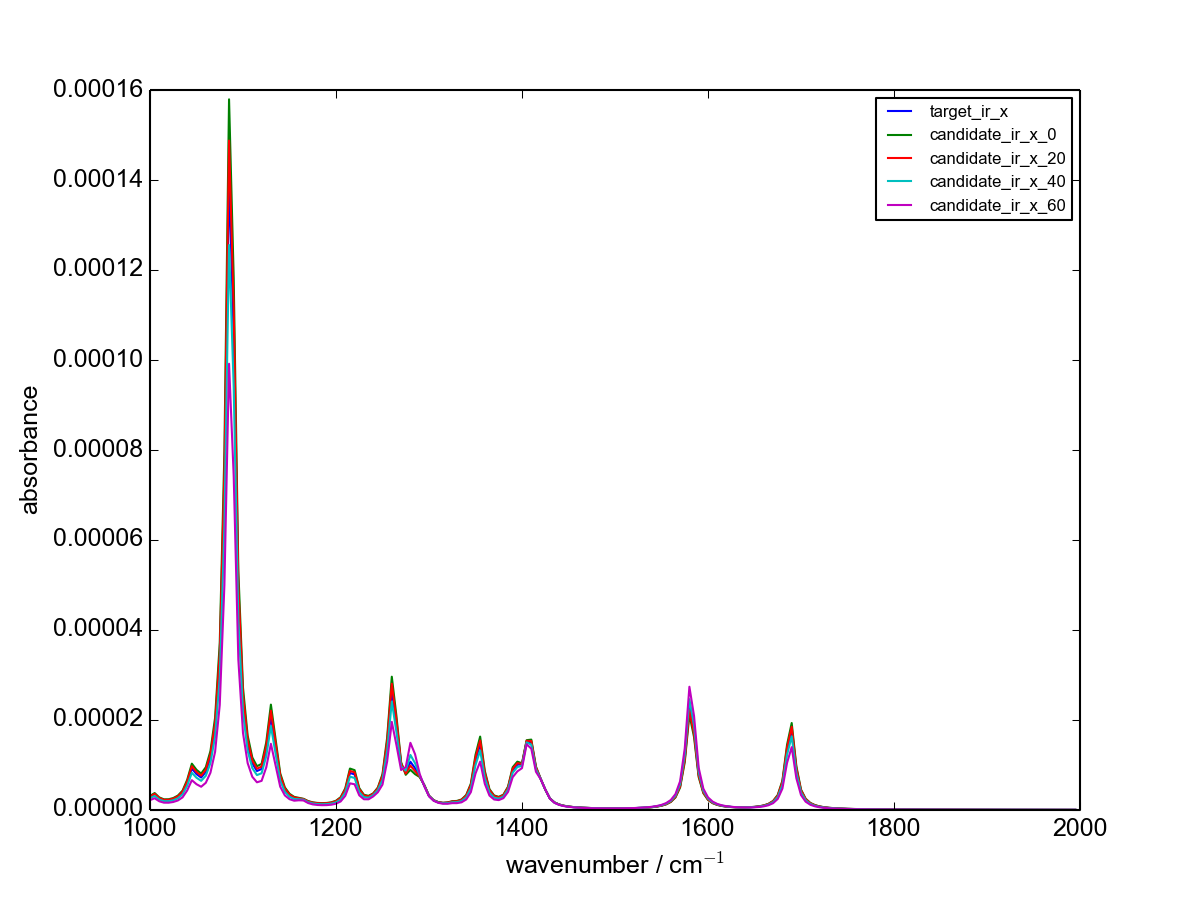
\includegraphics[scale=0.5]{Figures/Met_candidates_plotting_ir_x.png}
\caption{IR $x$-polarized spectra of methionine's four candidates and target. The candidates are with $\theta$ of $0^{\circ}$, $20^{\circ}$, $40^{\circ}$ and $60^{\circ}$. The target is produced by combining $10\%$ of $candidate\_ir\_x\_0$, $50\%$ $candidate\_ir\_x\_20$ and $40\%$ $candidate\_ir\_x\_40$. } \label{fig:2.2}
\end{figure}

\begin{figure}[!ht]
\centering
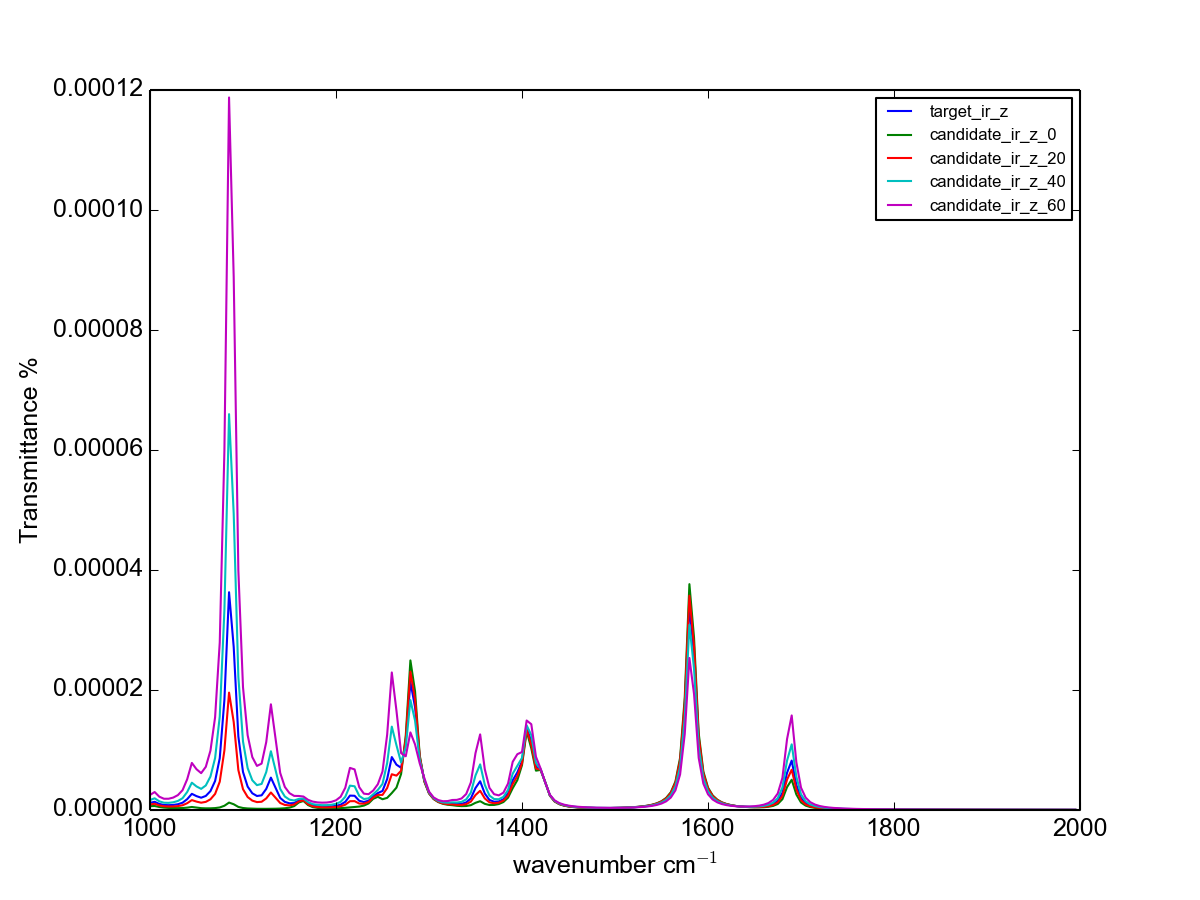
\includegraphics[scale=0.5]{Figures/Met_candidates_plotting_ir_z.png}
\caption{IR $z$-polarized spectra of methionine's four candidates and target. The candidates are with $\theta$ of $0^{\circ}$, $20^{\circ}$, $40^{\circ}$ and $60^{\circ}$. The target is produced by combining $10\%$ of $candidate\_ir\_x\_0$, $50\%$ $candidate\_ir\_x\_20$ and $40\%$ $candidate\_ir\_x\_40$.} \label{fig:2.3}
\end{figure}

\begin{figure}[!ht]
\centering
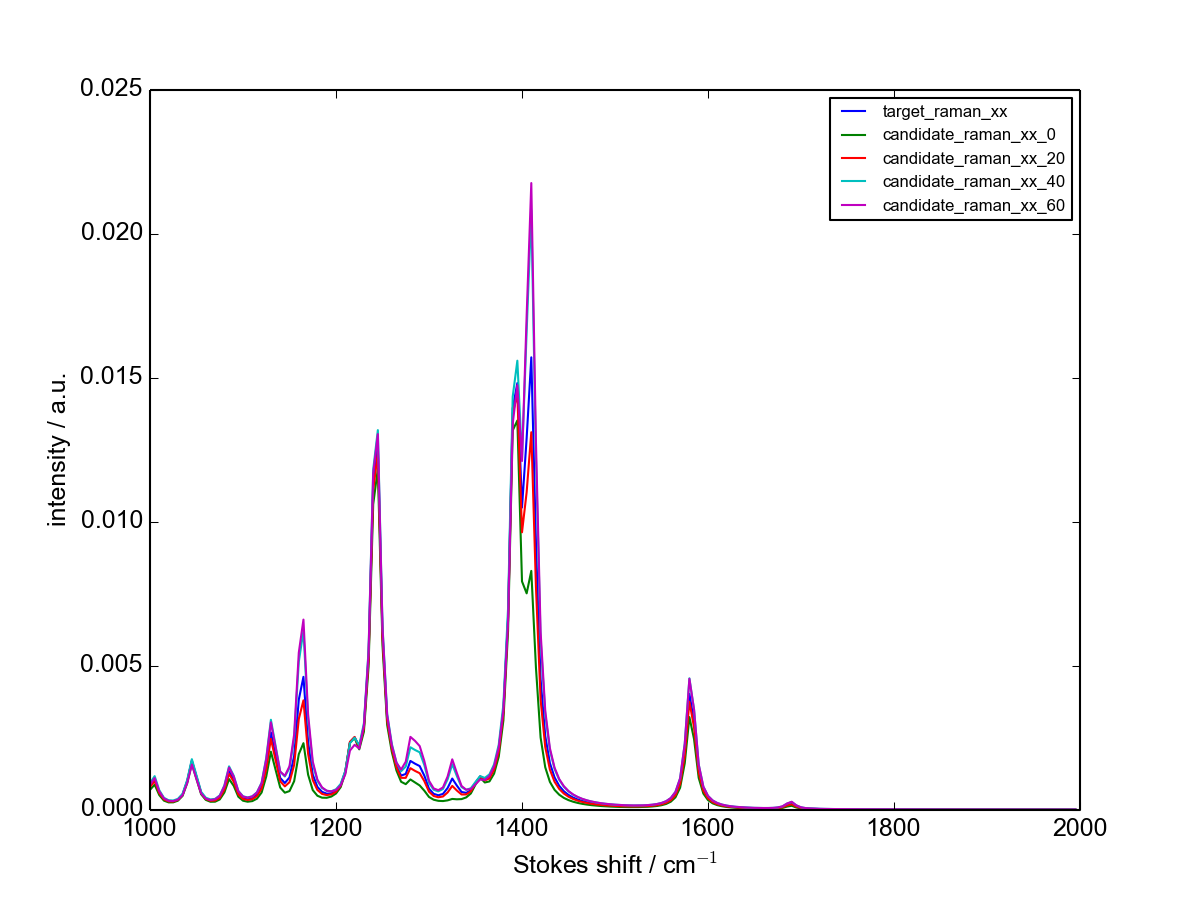
\includegraphics[scale=0.5]{Figures/Met_candidates_plotting_raman_xx.png}
\caption{Raman $xx$-polarized spectra of methionine's four candidates and target. The candidates are with $\theta$ of $0^{\circ}$, $20^{\circ}$, $40^{\circ}$ and $60^{\circ}$. The target is produced by combining $10\%$ of $candidate\_ir\_x\_0$, $50\%$ of $candidate\_ir\_x\_20$ and $40\%$ of $candidate\_ir\_x\_40$.} \label{fig:2.4}
\end{figure}

\begin{figure}[!ht]
\centering
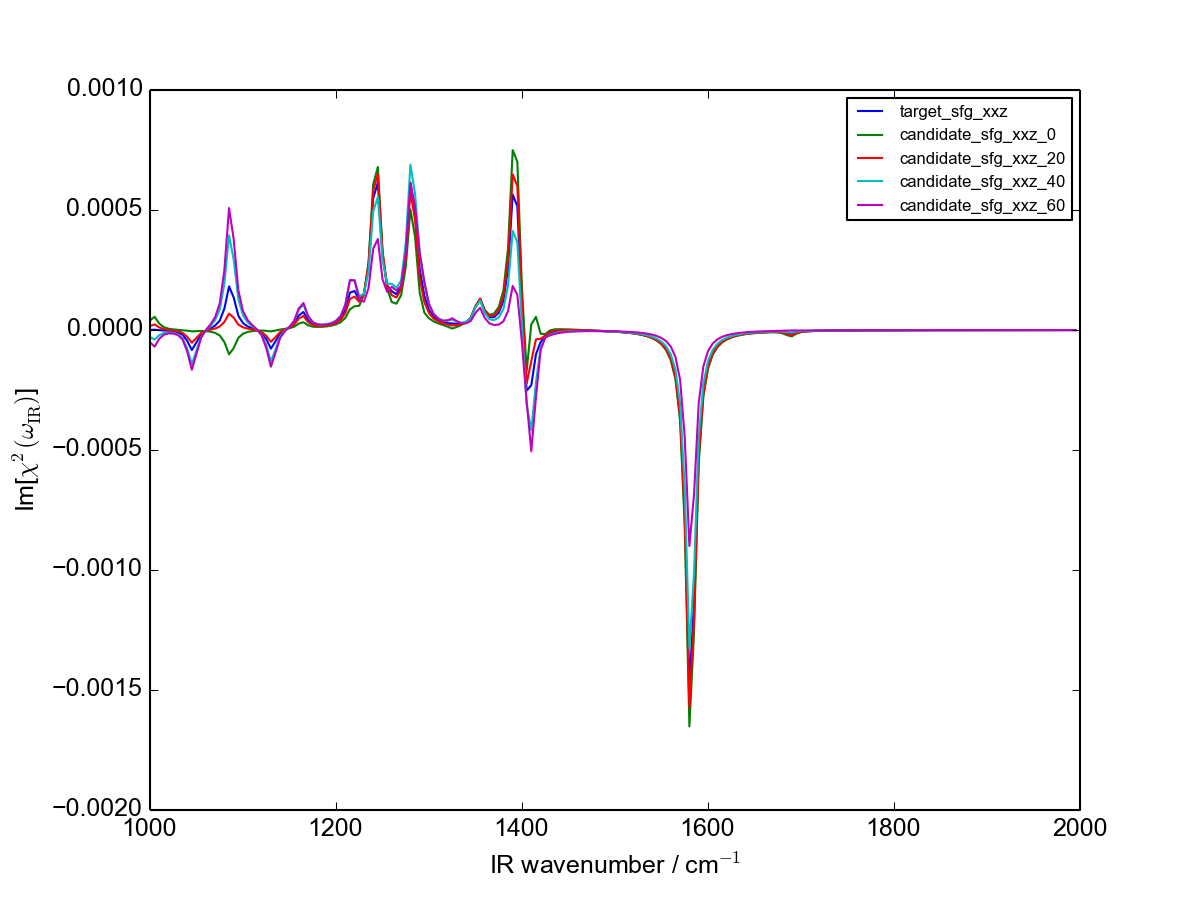
\includegraphics[scale=0.5]{Figures/Met_candidates_plotting_sfg_xxz.png}
\caption{SFG $xxz$-polarized spectra of methionine's four candidates and target. The candidates are with $\theta$ of $0^{\circ}$, $20^{\circ}$, $40^{\circ}$ and $60^{\circ}$. The target is produced by combining $10\%$ of $candidate\_ir\_x\_0$, $50\%$ of $candidate\_ir\_x\_20$ and $40\%$ of $candidate\_ir\_x\_40$.} \label{fig:2.5}
\end{figure}

\section{Conclusion}
Chapter \ref{ch:2} briefly explains what the current approaches are to extract molecular orientation distribution at surfaces, the molecular structures of six amino acids, and how to produce IR, Raman and SFG spectra theoretically. In Chapter \ref{ch:3}, our LP model is described and its properties are studied. It is conducted by using a simplified molecular model to gain an insight of our approach. The motivation of creating a simplified molecular model is to create a molecule as simple as possible that will allow us to study the properties of the LP model for this basic case. Information gained in Chapter \ref{ch:3} allows us to then study the approach using molecules in Chapters \ref{ch:4}, \ref{ch:5} and \ref{ch:6}.
	\startchapter{Simplified Molecular Model} \label{ch:3}

\section{Description}
The goal of Chapter \ref{ch:3} is to introduce the formulas used to describe our LP model. As well as exploring the properties of our LP model by using a toy molecule. This toy molecule contains limited vibration modesf. By doing so, the nature of the LP model we use to study the spectral information can be carefully analyzed. Our goal is to figure out with the the spectral information available, could LP model we use output any valuable information. \\

The toy molecule contains $4$ vibration modes. Theses vibrational peaks are at frequencies of $2850, 2960, 3050$ and $3200$. The widths of the peaks are $5, 10, 5$ and $15~cm^{-1}$, respectively. The amplitudes of the peak are $1, 0.7, -0.2$ and $0.5~cm^{-1}$, respectively. The comparing angles of the peaks are $15, 90, 0$ and $60$. (TODO: check with Dennis, how to further explain those comparing angles?)  \\

For the toy model, only IR spectroscopy is considered. Because we want to limit the complication that comes from the parameters needed to describe the real molecules. Equation \ref{eq:3.1} is used to generate the $cosine$-polarized IR spectrum. Both $\phi$ and $\psi$ Euler angles are integrated, only the difference on angle $\theta$ is considered. \\

\begin{eqnarray} \label{eq:3.1}
& f_{\theta}(x) = \displaystyle\sum^{4}_{q=1} A_q^2 * cos^2(\theta - \theta_q)\frac{\gamma^2}{(x- \omega_{\rm q})^2 + \gamma^2} 
\end{eqnarray}
where $A$ is the amplitude, $\theta_{q}$ is the comparing angle, $\gamma$ is the width, and $\omega_{\rm q}$ is the frequency. (TODO: Double check the correct meaning of each symbol) Ten candidates are produced with $10$ different $\theta$ values as follows: $0^{\circ}$, $10^{\circ}$, $20^{\circ}$, $30^{\circ}$, $40^{\circ}$, $50^{\circ}$, $60^{\circ}$, $70^{\circ}$, $80^{\circ}$, $90^{\circ}$. Their spectra are shown in Figure \ref{fig:3.1}. The 10 candidates have peaks at the same frequencies. The spectral signal for candidates is comparatively strong at each peak. \\

\begin{figure}[!ht] 
\centering
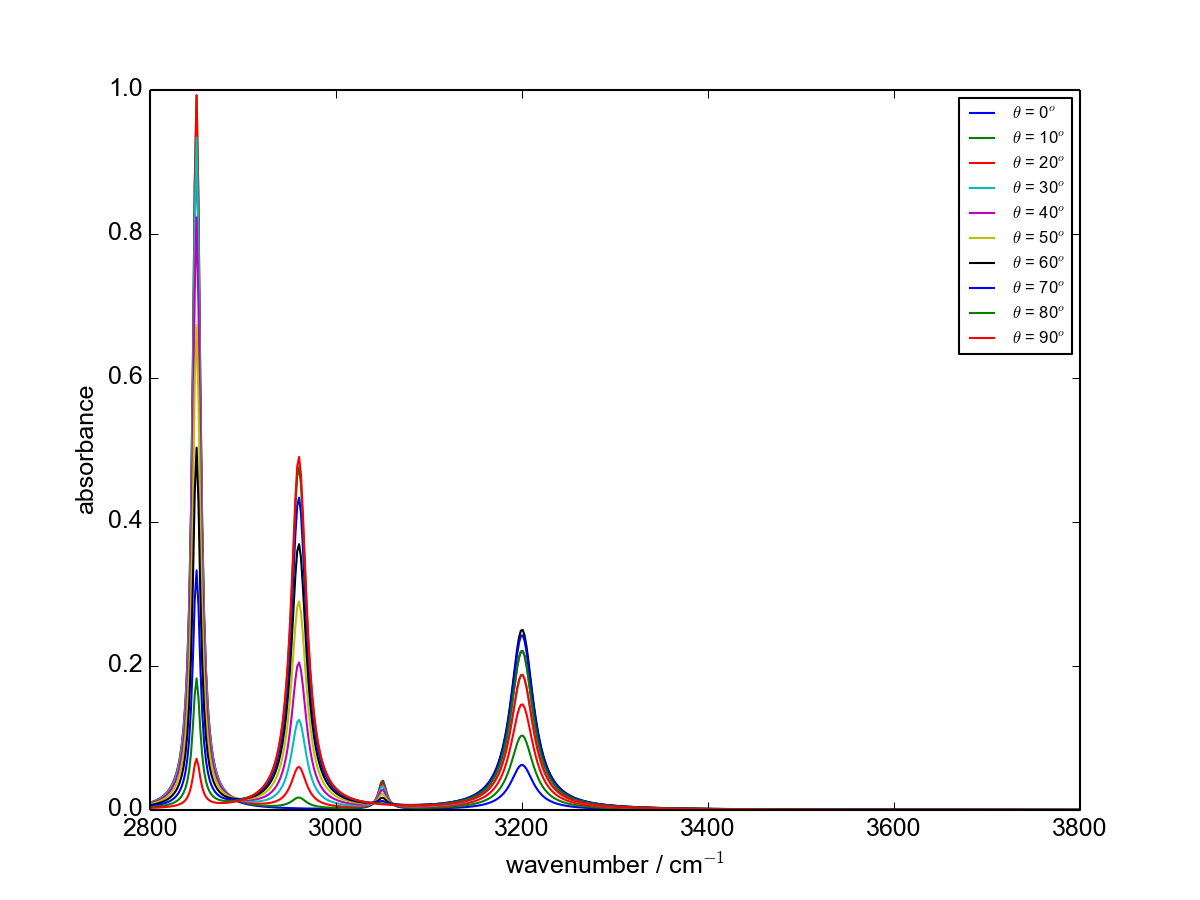
\includegraphics[scale=0.4]{Figures/Toy_Model_IR_Cosine_Projection.png} 
\caption{$cosine$- polarize IR spectra of toy model candidates} \label{fig:3.1}
\end{figure}

%A target spectrum is composed by combining $15$ percent of candidate with $\theta$ of $20^{\circ}$ and $85$ percent of candidate of $\theta$ of $70^{\circ}$: $0.15*f_{20}(x) + 0.85*f_{70}(x)$ in the following experiment. \\

\section{Linear Programming Model for Spectral Study}

Equation \ref{eq:3.2} is used to construct our LP model. The optimal solution returned by the LP solver is then compared with the target composition to see if they matches each other. This equation has also been used to study the composition of Ribonucleic acid (RNA) with ultraviolet (UV) spectra \cite{NYAS:NYAS900} and other UV spectroscopy studies  \cite{LPATUAS} back in the 60s. \\

\begin{eqnarray} \label{eq:3.2}
& \underset{p_{c}} {\text{minimize}} \displaystyle\sum^{\#~points}_{n=1} \left| Target- \displaystyle\sum^{\#~candidates}_{c=1}p_{c}f_{\theta}(x) \right| 
\end{eqnarray}
where $p_{c}$ are the unknown percentages for each candidate, which are the decision variables. $n$ is the number of points selected along the wavenumber, both for candidates and target spectra. $Target$ refers to the corresponding data points selected in target spectra. For each data point, the absolute residual between the target spectrum and the one composed by the decision variables is calculated. The objective function minimizes the sum of the absolute residuals over all the data points. \\

Because Equation \ref{eq:3.2} subjects to no restrictions, and the objection function is not in standard form. Getting rid of the absolute signs in the objective function is needed in order to use an LP approach. To eliminate the absolute sign is achieved by introducing one more variable $X$ and two more constraints for each data point as shown in Equation \ref{eq:3.3}. Then the previous model in Equation \ref{eq:3.2} is converted into the one in Equation \ref{eq:3.4} that can be solved by an LP solver. At last, one more constraint is introduced to restrict the sum of the percentages to be 1, as shown in Equation \ref{eq:3.4}. \\

For each point in the range of valid wavenumbers:
\begin{eqnarray} \label{eq:3.3}
& X = \left| Target-\displaystyle\sum^{\#~candidates}_{c=1}p_{c}f_{\theta}(x) \right| \nonumber \\
&  X \geq Target-\displaystyle\sum^{\#~candidates}_{c=1}p_{c}f_{\theta}(x)   \nonumber \\
& X \geq -Target+\displaystyle\sum^{\#~candidates}_{c=1}p_{c}f_{\theta}(x)  
\end{eqnarray} 

\begin{eqnarray} \label{eq:3.4}
& minimize \displaystyle\sum^{\#~points}_{n=1} X_p \nonumber \\
& X_1 - Target_1 + \displaystyle\sum^{\#~candidates}_{c=1}p_{c}f_{\theta}(x_1) \geq 0 \nonumber \\
& X_1 + Target_1 - \displaystyle\sum^{\#~candidates}_{c=1}p_{c}f_{\theta}(x_1) \geq 0 \nonumber \\
& ... \nonumber \\
& X_n - Target_n + \displaystyle\sum^{\#~candidates}_{c=1}p_{c}f_{\theta}(x_n) \geq 0 \nonumber \\
& X_n + Target_n - \displaystyle\sum^{\#~candidates}_{c=1}p_{c}f_{\theta}(x_n) \geq 0 \nonumber \\
& \displaystyle\sum^{\#~candidates}_{c=1}p_{c} = 1 
\end{eqnarray} 

Note that our LP model exactly describes our problem to be solved. Assuming that we can obtain sufficiently precise data, solving the LP will yield the target composition. Recall if the solution space is feasible and bounded, then there is a unique optimum solution. \\

\section{Linear Programming Model Implementation}

Next, we describe how to solve Equation \ref{eq:3.4} by implementing our LP model. Code is written to generate a file that contains all the candidates' spectral information needed for the experiments. For this step, the molecular properties files are used. For a specific candidate, given a molecular properties file and a $\theta$ value, the candidate's spectral information is obtained. For toy model, only the value of $\theta$ is needed, then Equation \ref{eq:3.1} is used to synthesize the spectral information. To further illustrate, a candidate class is written. This class defines candidate's $x$- and $z$-polarized IR spectra; $xx$-, $xy$-, $xz$-, and $zz$-polarized Raman spectra; $yyz$-, $yzy$-, $zzz$-polarized SFG spectra. Given a candidate's molecular properties and a $\theta$ value, a instance of this specific candidate is created. For the toy model, it only contains IR spectral information. Therefore, one candidate only contains $cosine$- and $sine$-polarized IR spectra. \\

In the second step, more code is written to generate a target composition of a list of needed candidates. Then the target composition is used to generate the target spectra. The probe range, which is the range of the wavenumber, is from 2800 to 3300 for toy model. The probe arrange is from $2000$ wavenumber to $3000$ wavenumber for real molecules. The target spectral information is generated in the same text file as candidate's spectral information. Depends on the experiment setting, code can be used to generate text files that contain different spectral information. \\

In the third step, the LP model is constructed by using the spectral information text file generated in the second step. This part of the code was written by Hung \cite{KuoKaiHung:Thesis:2015}. It reads all the candidates and target spectral information, and builds the LP model as shown in Equation \ref{eq:3.4}, then creates CPLEX LP input file. \\

In the fourth step, we use LP solver ``GNU linear progarmming tool kit" (GLPK) to read the CPLEX LP input file, then obtain the result. \\

\section{Experiments}

In Experiment 1 and 2, $4$ candidates are selected, the detailed setting is shown in Table \ref{tab:3.1}. In Experiment 1, there are $4$ candidates with $\theta$ of $0^{\circ}, 10^{\circ}, 20^{\circ}$, and $30^{\circ}$. In Experiment 2, the four candidates are with $\theta$ values of $0^{\circ}, 5^{\circ}, 10^{\circ}$, and $15^{\circ}$. Instead of having a $10$ degree variance in $\theta$, $5$ degree difference is applied on $\theta$ in Experiment 2. This means that when the candidates become more similar to each other than the ones in Experiment 1 as their spectra are more similar. In both experiments, 100 data points are selected evenly along the wavenumber from the spectra of $cosine$-polarized IR. The target composition of the candidates are the same for both experiments. In Experiment 1, the return composition is the same as the target one, however, the return composition for Experiment 2 does not match the target one. \\

\begin{table} 
\begin{center}
\begin{tabular}{| l | l | l | }
\hline
Experiment index & 1 & 2  \\
\hline
Number of Candidates & 4 & 4  \\
\hline
Candidates & [0, 10, 20, 30] & [0, 5, 10, 15] \\
\hline
Target Composition & [0.1, 0.5, 0.4, 0] & [0.1, 0.5, 0.4, 0]     \\
\hline
Number of Data Points & 100 from $cosine$-polarized IR &  100 from $cosine$-polarized IR     \\
\hline
Return Composition & [0.1, 0.5, 0.4, 0] & [0, 0.796962, 0.103038, 0.1] \\
\hline
\end{tabular} 
\end{center}
\caption{Experiment 1 and 2 setting using toy model}
\label{tab:3.1}
\end{table}	

In order to figure out why the return composition in Experiment 2 is different from the target one, the spectra generated by the return composition is plotted together with the target spectra as shown in Figure \ref{fig:3.2}. Note that the result spectra is almost identical to the target one. The residual between them is almost $0$. In order to see whether this observation is a general case, Experiment 3 is set up in Table \ref{tab:3.2}. Experiment 3 contains more candidates than Experiments 1 and 2. $10$ candidates are included with $\theta$ values ranging from $0^{\circ}$ to $90^{\circ}$.  \\

\begin{figure}[!ht] 
%\centering
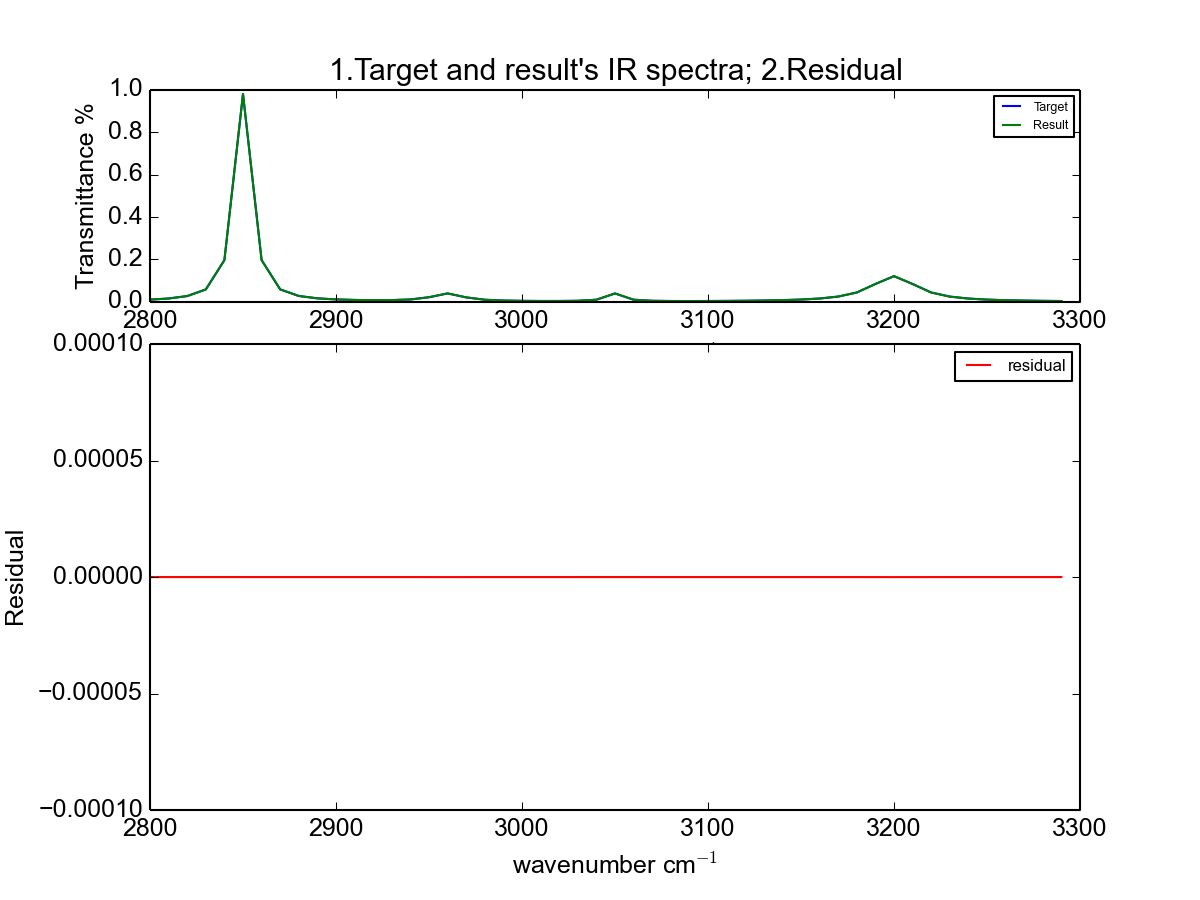
\includegraphics[scale=0.7]{Figures/toy_model_result_plotting_ir_cos_4candi_1.png}
\caption{Toy model Experiment 2 resulting $cosine$-polarized IR spectrum plotted with the target spectrum; and the residual plot between the spectra.}
\label{fig:3.2}
\end{figure}

\begin{table} 
%\begin{center}
\begin{tabular}{| l | p{7cm} | }
\hline
Experiment index & 3  \\
\hline
Number of Candidates & 10   \\
\hline
Candidates & [0, 10, 20, 30, 40, 50, 60, 70, 80, 90]  \\
\hline
Target Composition & [0.1, 0, 0.5, 0, 0.4, 0, 0, 0, 0, 0] \\
\hline
Number of Data Points & 100 from $cosine$-polarized IR \\
\hline
Return Composition & [0, 0, 0.730541, 0, 0.212061,0, 0, 0.0573978, 0, 0] \\
\hline
\end{tabular}
%\end{center}
\caption{Experiment 3 setting of toy model}
\label{tab:3.2}
\end{table}	

\begin{figure}[!ht] 
\centering
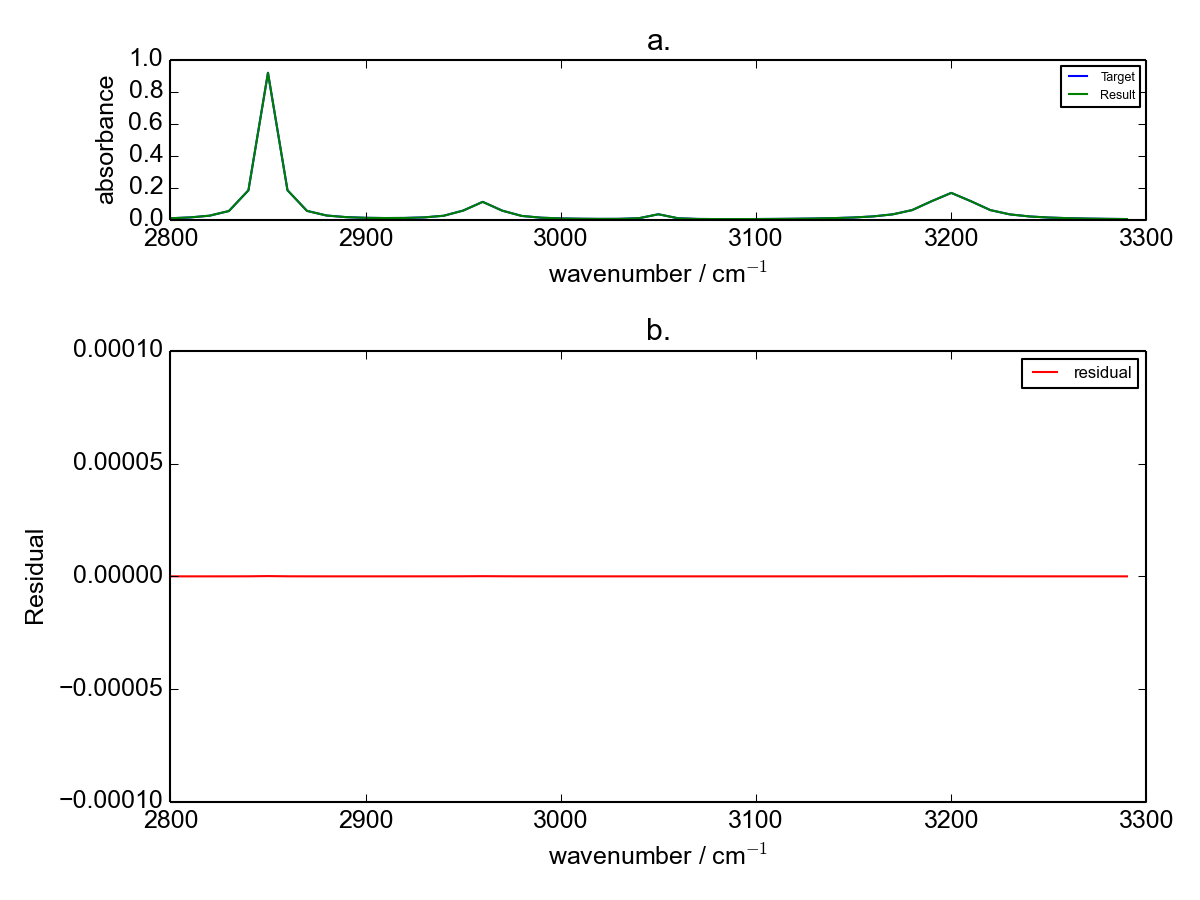
\includegraphics[scale=0.7]{Figures/toy_model_result_plotting_ir_cos_10candi_1.png} 
\caption{Toy model Experiment 3 resulting $cosine$-polarized IR spectrum plotted with target spectrum; and the residual plot between the two spectra}
\label{fig:3.3}
\end{figure}

Table \ref{tab:3.2} indicates the return composition of Experiment 3 is different from the target one. Figure \ref{fig:3.3} shows that the spectrum produced by the return composition is almost identical to the one generated by the target composition in Experiment 3. The residual is negligible as well. This observation is the same as Experiment 2. \\

Among Experiment 1, 2 and 3, only the return composition of Experiment 1 matches its target one. However, in Experiment 2, the difference in $\theta$ value among the candidates is smaller than Experiment 1. In Experiment 3, the number of the candidates is larger than Experiment 1. Both effects increase the complexity of the experiments. In both Experiment 2 and 3, the spectrum constructed by the return composition matches to the one built by the target composition. \\

The above observation demonstrates that there are multiple compositions can achieve in constructing the spectrum that are close to the target one. The numerical limitation helps the LP solver to converge to a unique optimum solution. The reason for Experiment 1 to return a composition that matches to the target one, is that the spectral information used to construct the LP model is competent. The constraints constructed in the LP model of Experiment 1 eventually converge to the target composition. \\ 

In order to add necessary information to construct the constraints in our LP model, IR's second polarization is introduced to the toy model: the $sine$ polarization. Figure \ref{fig:3.4} describes how the $sine$-polarized spectra presented for $10$ candidates. Experiment 4 and 5 include both polarizations' spectral information in the LP model. In Table \ref{tab:3.3}, Experiment 4's setting is based on Experiment 2, with $sine$-polarized IR spectral information added. $100$ data points are selected from this additional spectrum, then converted to additional decision variables and constraints in the LP model. Experiment 5, it is based on Experiment 3, with $sine$-polarized IR spectral information added. In both Experiment 4 and 5, the return composition matches to the target one. This further proves that as long as we have sufficing information for our LP model, the LP solver returns a composition matches to the target one. \\ 

\begin{figure}[!ht]
\centering
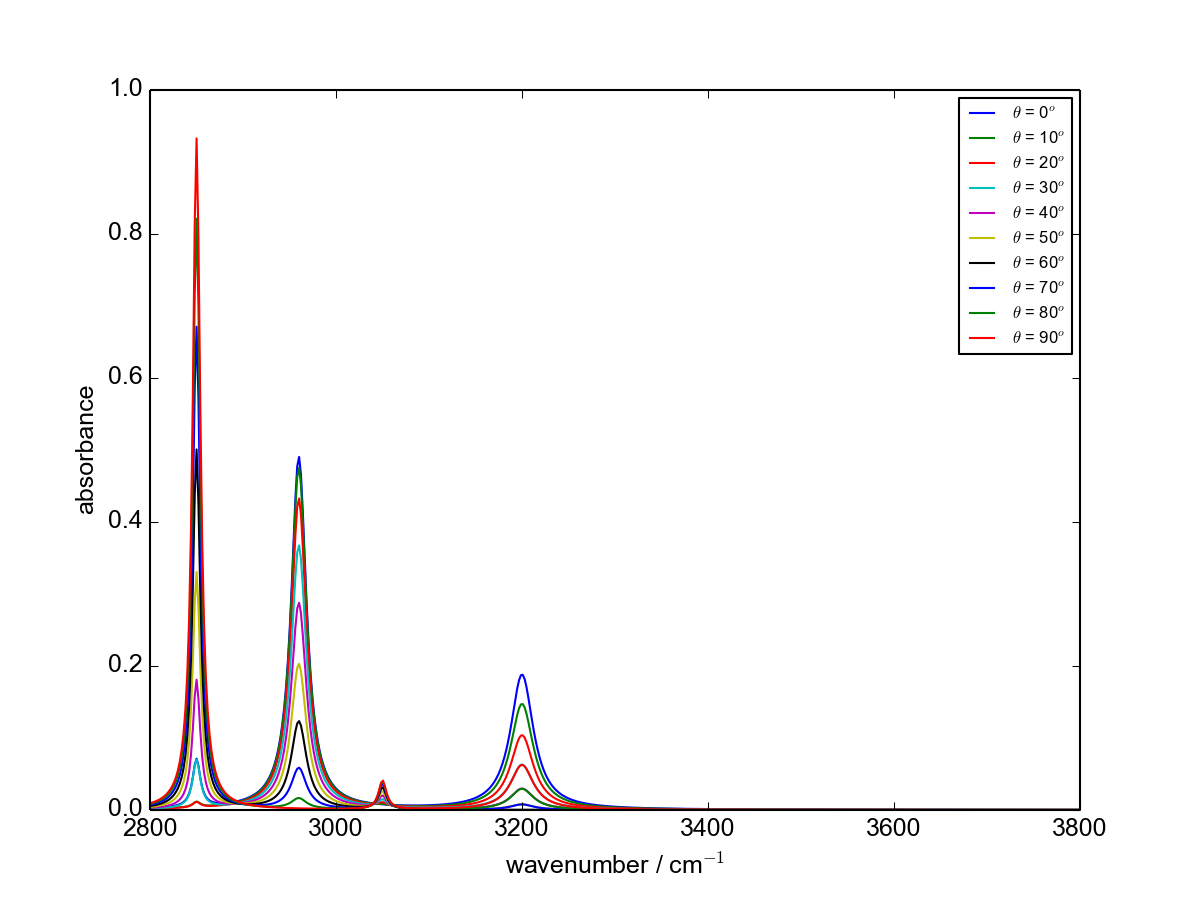
\includegraphics[scale=0.7]{Figures/Toy_Model_IR_Sine_Projection.png} 
\caption{$sine$-polaried IR spectra of toy model candidates with $\theta$ value expanded from $0^{\circ}$ to $90^{\circ}$}  \label{fig:3.4}
\end{figure}

\begin{table} \small 
\begin{center}
\begin{tabular}{| l | p{5cm} | l |}
\hline
Experiment index & 4 & 5\\
\hline
Number of Candidates & 4 & 10 \\
\hline
Candidates & [0, 5, 10, 15] & [0, 10, 20, 30, 40, 50, 60, 70, 80, 90] \\
\hline
Target Composition & [0.1, 0.5, 0.4, 0] & [0.1, 0, 0.5, 0, 0.4, 0, 0, 0, 0, 0]\\
\hline
Number of Data Points & 100 from $cosine$-polarized IR + 100 from $sine$-polarized IR & 100 from $cosine$-polarized IR + 100 from $sine$-polarized IR\\
\hline
Return Composition & [0.1, 0.5, 0.4, 0] & [0.1, 0, 0.5, 0, 0.4, 0, 0, 0, 0, 0] \\
\hline
\end{tabular} 
\caption{Experiment 4 and 5 setting of toy model}\label{tab:3.3}
\end{center}
\end{table}		

\section{Constraint Study Based on Experiment 4}

From Experiment 1 to 5 of toy model, we know having sufficient information in our LP model is the key to obtain the target composition. Having sufficient information means having enough constraints to help LP model converge to a desired result. The information is coming from the valuable data points selected along the spectra. This leads us to do a more detailed study on the constraints in order to see how many data points are enough to get the desired composition.\\ 

Based on Experiment 4, experiments about formulating the LP model with different data information are conducted in Table \ref{tab:3.4}. The number of data points indicates how many data points are selected. Points Selection shows how data points are selected. For example, [2800, 3300, 50] means along wavenumber from 2500 to 3300, every 50 wavenumber a data point is selected along a spectrum. $cosine$ and $sine$ indicate the corresponding polarization of IR spectrum. \\

\begin{table} \small
\begin{center}
\begin{tabular}{| p{3cm} | p{3cm} | p{5cm} | l |} \hline
	Experiment \# & \# Data Points & Points Selection & Return Composition \\ \hline
	6 & 10 & [2800, 3300, 50], $cosine$ & [0, 0.796962, 0.103038, 0.1] \\ \hline
	7 & 20 & [2800, 3300, 25], $cosine$ & [0, 0.796962, 0.103038, 0.1] \\ \hline
	8 & 25 & [2800, 3300, 20], $cosine$ & [0, 0.796962, 0.103038, 0.1] \\ \hline
	9 & 32 & [2800, 3300, 15], $cosine$ & [0, 0.796962, 0.103038, 0.1] \\ \hline
	10 & 50 & [2800, 3300, 10], $cosine$ & [0, 0.796962, 0.103038, 0.1] \\ \hline
	11 & 100 & [2800, 3300, 5], $cosine$ & [0, 0.796962, 0.103038, 0.1] \\ \hline
	12 & $100 + 1$ & [2800, 3300, 5], $cosine$ \newline [2800, 3300, 500], $sine$ & [0, 0.796962, 0.103038, 0.1] \\ \hline
	13 & $100 + 5$ & [2800, 3300, 20], $cosine$ \newline [2800, 3300, 100], $sine$ & [0, 0.796962, 0.103038, 0.1] \\ \hline
	14 & $100 + 10$ & [2800, 3300, 20], $cosine$ \newline  [2800, 3300, 50], $sine$ & [0, 0.796962, 0.103038, 0.1] \\ \hline
	15 & $100 + 50$ & [2800, 3300, 20], $cosine$ \newline  [2800, 3300, 10], $sine$ & [0.1, 0.5, 0.4, 0] \\ \hline
	16 & $100 + 100$ & [2800, 3300, 20], $cosine$ \newline  [2800, 3300, 5], $sine$ & [0.1, 0.5, 0.4, 0] \\ 
	\hline
\end{tabular} 
\end{center}
\caption{Constraint study based on Experiment 4} \label{tab:3.4}
\end{table}

As Table \ref{tab:3.4} indicates, the return compositions of Experiment 6 to 14 are the same. To the contrary, from Experiment 15, the return composition matches the target one. In Figure \ref{fig:3.5} displays the spectra conducted by $[0, 0.796962, 0.103038, 0.1]$ and $[0.1, 0.5, 0.4, 0]$, both $sine$- and $cosine$-polarized IR spectra generated by these two compositions are identical.

\begin{figure}[!ht] 
\centering
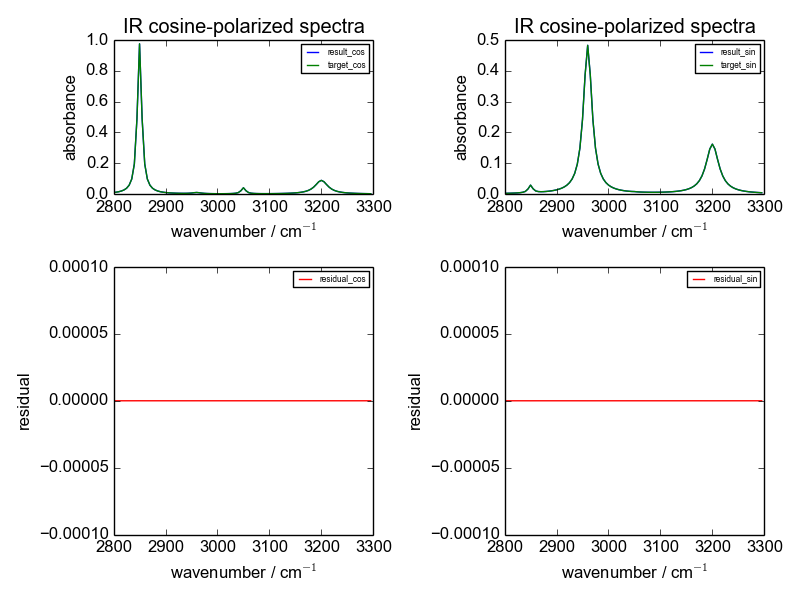
\includegraphics[scale=0.3]{Figures/toy_model_result_plotting_ir_sin_4candi_constraint_study_experiment4.png} 
\caption{IR spectra plotted by the return compositions from the constraint study based on Experiment 4 of toy model}\label{fig:3.5}
\end{figure}


\section{Constraint Study Based on Experiment 5}

Based on Experiment 5, similar constraint study is conducted as displayed in Table \ref{tab:3.5}, and the same observation is obtained as the experiments in Table \ref{tab:3.4}. When the result composition $[0, 0, 0.730541, 0, 0.212061,0, 0, 0.0573978, 0, 0]$ and target one $[0.1, 0, 0.5, 0, 0.4, 0, 0, 0, 0, 0]$ are used to plot the spectra, the produced spectra are almost identical as shown in Figure \ref{fig:3.6}.

\begin{table} \tiny 
\begin{center}
\begin{tabular}{| p{2cm} | p{2cm} | p{4cm}  | l |}
\hline
Experiment \# & \# of Data Points & Point Selection & Return Composition \\ \hline
17 & 10 & [2800, 3300, 50], $cosine$ & [0.156758, 0, 0, 0.825977, 0, 0, 0, 0, 0, 0.017265] \\ \hline
18 & 25 & [2800, 3300, 20], $cosine$ & [0, 0, 0.730541, 0, 0.212061, 0, 0, 0.0573978, 0, 0, 0] \\ \hline
19 & 50 & [2800, 3300, 10], $cosine$ & [0, 0, 0.730541, 0, 0.212061, 0, 0, 0.0573978, 0, 0, 0] \\ \hline
20 & 100 & [2800, 3300, 5], $cosine$ & [0, 0, 0.730541, 0, 0.212061, 0, 0, 0.0573978, 0, 0, 0] \\ \hline
21 & 500 & [2800, 3300, 1], $cosine$ & [0, 0, 0.730541, 0, 0.212061, 0, 0, 0.0573978, 0, 0, 0] \\ \hline	
22 & $100 + 1$ & [2800, 3300, 5], $cosine$ \newline [2800, 3300, 500], $sine$  & [0, 0, 0.730541, 0, 0.212061, 0, 0, 0.0573978, 0, 0, 0] \\ \hline
23 & $100 + 10$ & [2800, 3300, 5], $cosine$ \newline [2800, 3300, 50], $sine$  & [0.361587, 0, 0.312061, 0.326352, 0, 0, 0, 0, 0] \\ \hline
24 & $100 + 20$ & [2800, 3300, 5], $cosine$ \newline [2800, 3300, 25], $sine$  & [0.174023, 0, 0, 0.791447, 0, 0, 0.0345301, 0, 0, 0] \\ \hline
25 & $100 + 25$ & [2800, 3300, 20], $cosine$ \newline [2800, 3300, 20], $sine$  & [0.174023, 0, 0, 0.791447, 0, 0, 0.0345301, 0, 0, 0] \\ \hline
26 & $100 + 50$ & [2800, 3300, 5], $cosine$ \newline [2800, 3300, 10], $sine$  & [0, 0, 0.753209, 0, 0.146791, 0, 0.1, 0, 0, 0] \\ \hline
27 & $100 + 84$ & [2800, 3300, 5], $cosine$ \newline [2800, 3300, 6], $sine$  & [0.174023, 0, 0, 0.791447, 0, 0, 0.0345301, 0, 0, 0] \\ \hline
28 & $100 + 100$ & [2800, 3300, 5], $cosine$ \newline [2800, 3300, 5], $sine$  & [0.1, 0, 0.5, 0, 0.4, 0, 0, 0, 0, 0] \\ 
\hline
\end{tabular} \\
\caption{Constraint study based on Experiment 5 of toy model}\label{tab:3.5}
\end{center}
\end{table}

\begin{figure}[!ht] 
\centering
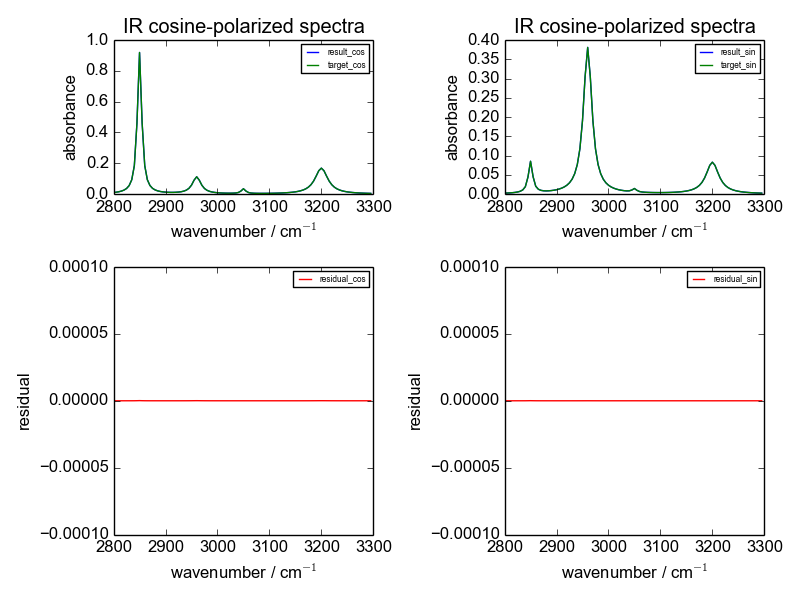
\includegraphics[scale=0.3]{Figures/toy_model_result_plotting_ir_sin_10candi_constraint_study_experiment5.png} 
\caption{IR spectra plotted by the return compositions from the constraint study based on Experiment 5 of toy model}\label{fig:3.6}
\end{figure}

\section{Discussion and Conclusion}

Recall that our LP model, for the right data set is expected to return the target composition. We can conclude that, if the target composition is not returned correctly, then the data we collect is not sufficient to describe the experiments to our LP model. \\

However, when the target composition is not returned correctly, the return composition does build spectra that are almost identical to the target ones. This means that there are more than one composition can build the spectra that are almost identical to the target ones. Because of the numerical limitation, an unique optimum solution is always obtained. \\

The above conclusion leaves us a new question: how do we know there is sufficient spectral information in order to obtain the target composition of candidates at interfaces? To answer this question, further experiments are conducted by applying the spectral information of real molecules to the LP model. The goal is to investigate with all the spectral information we can obtain for real molecules, can the LP model return the target composition of candidates at interfaces. If this goal can be achieved, can this approach be applied systematically to various circumstances?

%Above analysis simulates the following question: how can we know there is enough information to achieve the target composition? In the next step, we will experiment with real molecules. The goal is to investigate with all the spectral information that we can obtain for real molecules, can our LP model return the target composition for the target spectrum? If yes, can we apply the LP model systematically? Furthermore, to maximally explore the capacity of our LP model, and study its limitation. Finally, come up with some general instructions for applying our LP model. These are the main focus for the following chapters.\\

		

		 




	\startchapter{Generating Candidates based on Realistic Molecular Model} \label{ch:4}
\section{Description}

After experimenting with the simplified molecule, lacking sufficient spectral information is the key cause for the failure of obtaining the correct target composition. First of all, in the simplified molecule, there are only four vibrational modes, the spectral information is limited. Secondly, the similarity among the candidates is high, as all the candidates are coming from one same molecule. Third, only IR spectra is considered. \\

In this chapter, test cases are conducted using realistic molecules. In addition to IR, both Raman and SFG spectra are calculated for these molecules, which makes the study one step closer to the overall goal and scope. The realistic molecule focused on this chapter is Methionine amino acid. \\

Same as the simplified molecule, in order to limit the possible candidate space of Methionine, $twist$ and $azimuthal$ angular distributions are assumed to be isotropic, which are integrated. Only $\theta$ in Euler angles is considered in Methionine's surface orientation distribution function. In Chapter \ref{ch:2} section Generating model spectra, how a molecule's IR, Raman and SFG spectra are generated have been explained. Two unique IR spectra can be obtained from $x$, and $z$ polarizations. Four unique Raman spectra can be obtained from $xx$, $xy$, $xz$ and $zz$ polarizations. Three unique SFG spectra can be obtained from $xxz$, $xzx$ and $zzz$ polarizations.\\

The goal is to see if those spectral information is sufficient for the LP model to return the correct target composition of the candidates of one type molecule at interfaces. If yes, we need to figure out which spectral information is needed for the LP model. If no, we need to check if the cause of the failure is the same as the simplified molecule. \\

\section{Test Cases}

\begin{table} 
\begin{center}
\begin{tabular}{| l | l | l |  }
\hline
Test Case \# & 1 & 2 \\
\hline
\# Candidates & 4 & 4 \\
\hline
Candidates & [0, 20, 40, 60] & [0, 20, 40, 60] \\
\hline
Target Composition & [0.1, 0.5, 0.4, 0] & [0.1, 0.5, 0.4, 0] \\
\hline
\# Data Points & 200 $x$ & 200 $z$ \\
\hline
%Return Composition & [0.701654, 0, 0, 0.298346] & [0.701654, 0, 0, 0.298346] \\
Return Composition & [0.70, 0, 0, 0.30] & [0.70, 0, 0, 0.30] \\
\hline
\end{tabular} 
\end{center}
\caption{Test Case 1 and 2 setting for methionine candidates} 
\label{tab:4.1}
\end{table}	

\begin{table} 
\begin{center}
\begin{tabular}{| l | l | l | }
\hline
Test Case \# & 3 & 4 \\
\hline
\# Candidates & 4 & 4  \\
\hline
Candidates & [0, 20, 40, 60] & [0, 20, 40, 60]\\
\hline
Target Composition & [0.1, 0.5, 0.4, 0] & [0.1, 0.5, 0.4, 0]\\
\hline
\# Data Points & 200 $x$ + 200 $z$ & 200 $x$ + 200 $xx$\\
\hline
%Return Composition & [0.701654, 0, 0, 0.298346] & [0.1, 0.5, 0.4, 0]\\
Return Composition & [0.70, 0, 0, 0.30] & [0.1, 0.5, 0.4, 0]\\
\hline
\end{tabular} 
\end{center}
\caption{Test Case 3 and 4 setting for methionine candidates} 
\label{tab:case3and4}
\end{table}	

In Table \ref{tab:4.1} and \ref{tab:case3and4}, four test cases are set up with four candidates and same target composition. These four candidates have $\theta$ of the following degree: $0^{\circ}$, $20^{\circ}$, $40^{\circ}$ and $60^{\circ}$. The only difference among these four test cases is the spectroscopy information we select to apply to the LP model, and it is indicated by the Number of Data Points. In Case 1, only $x$-polarized IR spectral information is used. This means that only data points from $x$-polarized IR are selected to apply to the LP model. Same for Case 2, data points are obtained from spectra of IR's $z$-polarized IR. In Test Case 3, the spectral information of $x$ and $z$-polarized IR are combined. At last, in Case 4, spectral information of $x$-polarized IR and $xx$-polarized Raman are combined. Case 4 contains the most abundant information, as its return composition matches to the target one. \\

When merely using IR information, the return composition is the same for Case 1, 2 and 3. Figure \ref{fig:4.1} displays the resulting spectra generated by using the return composition obtained from the first three test cases. The resulting spectra is almost identical to the target ones. It indicates that with only IR spectral information is not sufficient to get the target composition.  However, the spectra built by the return composition matches the target spectra. This means that further information is needed to build the constraints of the LP model. The more constraints are introduced, the more accurate the return composition will be. \\

\begin{figure}[!ht]
\centering
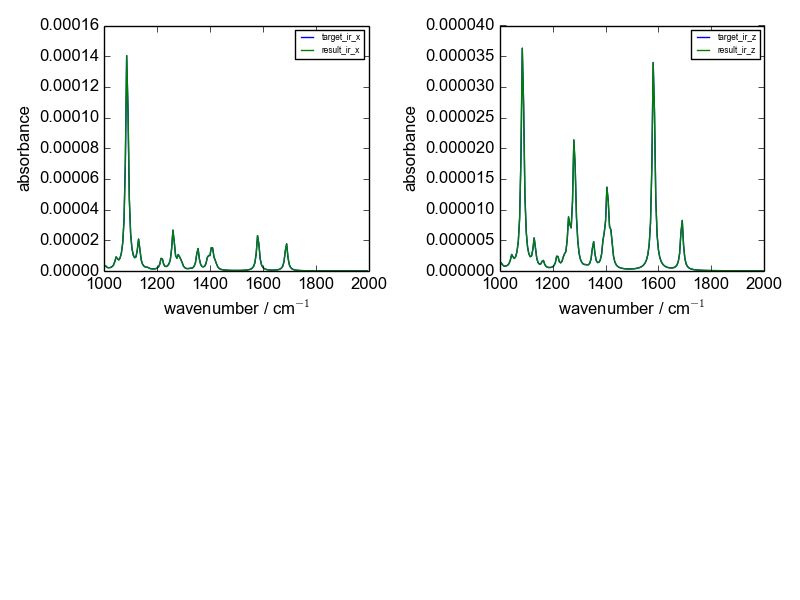
\includegraphics[scale=0.7]{Figures/ir_xz_result_plotting.png}
\caption{Compare target IR spectra with the ones generated by the return composition of Case 1, 2 and 3}  \label{fig:4.1}
\end{figure}

In Case 4, combining IR and Raman spectral information is sufficient to obtain the target composition. When the difference in $\theta$ degree for candidates decreases from $20^{\circ}$ to $10^{\circ}$. Checking if Raman and IR together is still sufficient to derive the target composition is desired. Therefore, the following test cases are conducted as shown in Table \ref{tab:4.2}. \\

\begin{table} \tiny 
\resizebox{\textwidth}{!}{
\begin{tabular}{| l | p{3cm} | l | l |}
\hline
\# Candidates & \multicolumn{2}{l|}{4} \\ \hline
Candidates & \multicolumn{2}{l|}{[0, 10, 20, 30]} \\ \hline
Target Composition & \multicolumn{2}{l|}{[0.1, 0.5, 0.4, 0]} \\ \hline
Test Case index & \# Data Points & Result Composition \\ \hline
%5 & 200 $x$ \newline 200 $z$ & [0.752528, 0, 0, 0.247472]  \\ \hline
5 & 200 $x$ \newline 200 $z$ & [0.75, 0, 0, 0.23]  \\ \hline
6 & 200 $x$  \newline 200 $z$ \newline 200 $xx$& [0.1, 0.5, 0.4, 0] \\ \hline
7 & 200 $xx$ \newline 200 $xy$ \newline 200 $xz$& [0.1, 0.5, 0.4, 0] \\ \hline
8 & 200 $xx$ \newline 200 $xy$ \newline 200 $zz$ & [0.1, 0.5, 0.4, 0] \\ \hline
9 & 200 $xx$ \newline 200 $xy$ \newline 200 $xz$ \newline 200 $zz$& [0.1, 0.5, 0.4, 0] \\ \hline
\end{tabular} 
%\end{center}
}
\caption{Test case 5 to 9 setting for methionine candidates}
\label{tab:4.2}
\end{table}	

Case 5 shows that the LP model constructed by merely using IR spectral information is not sufficient to derive the target composition. Case 6 indicates that combining IR and Raman spectral information helps to derive the target composition. What's more, Case 7, 8 and 9, illustrate that Raman spectral information itself is sufficient to obtain the target composition as well. \\

For test case setting in Table \ref{tab:4.1}, \ref{tab:case3and4} and \ref{tab:4.2}, combining IR and Raman spectral information to construct a LP model is sufficient enough to obtain the target composition. In order to study the limitation of the LP model, the complexity of the test case setting needed to be increased. Therefore, another group of test cases are designed as shown in Table \ref{tab:4.3}. There are 5 candidates included in the test cases. Each candidate has $\theta$ with the following degree: $0^{\circ}$, $10^{\circ}$, $20^{\circ}$, $30^{\circ}$ and $40^{\circ}$. The target composition is more complex than previous test cases, each candidate takes 20\% in the mixture. \\

Case 10 applys only IR spectral information to the LP model, and the return composition does not match the target one. Case 11 uses only Raman spectral information, and the return composition does not match to the target neither. Same for Case 12 that uses only SFG spectral information. From Case 13, different kinds of spectral information are combined. In Case 13, IR and Raman spectral information is used to produce the LP model, still the return composition is different from the target one. Case 14 combines Raman and SFG, Case 15 uses IR and SFG, Case 16 cooperates all the three spectral information, however, none of them returns a composition that matches the target one. \\

The results of Case 10 to 16 indicate that even combining all the spectral information of IR, Raman and SFG, it is still not sufficient to attain the target composition for the test cases set up in Table \ref{tab:4.3}. The spectral information we apply to the LP model is showing its limitation in these test cases. In order to confirm the reason causing the LP model to returning the target composition is because of insufficient information, further test cases are conducted in Table \ref{tab:4.4}. \\

\begin{table} \tiny
\begin{center}
\resizebox{\textwidth}{!}{
\begin{tabular}{| l | p{3cm} | l | l |}
\hline
Number of Candidates & \multicolumn{2}{l|}{5} \\ \hline
Candidates & \multicolumn{2}{l|}{[0, 10, 20, 30, 40]} \\ \hline
Target Composition & \multicolumn{2}{l|}{[0.2, 0.2, 0.2, 0.2, 0.2]} \\ \hline
Test case index & Constraints & Result  \\ \hline
10 & 200 $x$ \newline 200 $z$& [0.61, 0, 0, 0, 0.40]  \\ \hline
11 & 200 $xx$ \newline 200 $xy$ \newline 200 $xz$ \newline 200 $zz$& [0.25, 0, 0.50, 0, 0.25]  \\ \hline
12 & 200 $xxz$ \newline 200 $xzx$ \newline 200 $zzz$& [0.32, 0, 0.31, 0.16, 0.21]  \\ \hline
13 & 200 $x$ \newline 200 $z$ \newline 200 $xx$ \newline 200 $xy$ \newline 200 $xz$ \newline 200 $zz$& [0.25, 0, 0.50, 0, 0.25]  \\ \hline
14 & 200 $xx$ \newline 200 $xy$ \newline 200 $xz$ \newline 200 $zz$ \newline 200 $xxz$ \newline 200 $xzx$ \newline 200 $zzz$& [0.32, 0, 0.31, 0.16, 0.21]  \\ \hline
15 & 200 $x$ \newline 200 $z$ \newline 200 $xxz$ \newline 200 $xzx$ \newline 200 $zzz$& [0.32, 0, 0.31, 0.16, 0.21]  \\ \hline
16 & 200 $x$ \newline 200 $z$ \newline 200 $xx$ \newline 200 $xy$ \newline 200 $xz$ \newline 200 $zz$ \newline 200 $xxz$ \newline 200 $xzx$ \newline 200 $zzz$& [0.32, 0, 0.31, 0.16, 0.2]  \\ \hline
\end{tabular} 
}
\end{center}
\caption{Test Case 10 to 16 setting for methionine candidates. For more precise result data refer Table \ref{tab:7.1}.} \label{tab:4.3}
\end{table}

\section{Test Cases to Explain the Limitation of LP Model for Methionine Molecule}

To further explore the reason that LP model reaches its limitation for the realistic molecule, Case 17 and 18 are conducted. To make the study case more general than Case 1 to 16, candidates' $\theta$ values are expanded from $0^{\circ}$ to $80^{\circ}$. In total, there are $9$ candidates. Because the SFG spectra for $\theta$ of $90^{\circ}$ is a straight line, it is excluded from all the test cases related to realistic molecules. For target composition, five candidates are randomly selected to be presented. The difference between Case 17 and 18 is that different amount of data points are selected to build the LP model. From all three spectroscopy techniques' spectral information, every 5 wavenumber a data point is selected for Case 17. Every 500 wavenumber a data point is selected for Case 18. As a result, Case 17 and 18 each returns a different composition. Both compositions do not match to the target one. \\

However, in both Case 17 and 18, when the return composition is used to generate the IR, Raman and SFG spectra, then these spectra are plotted together with the spectra created by the target composition. All the spectra are almost identical for IR, Raman and SFG. Figure \ref{fig:4.2}, \ref{fig:4.3} and \ref{fig:4.4} display the spectra plotted by using the return composition and the target one of Case 17. Every spectrum is almost identical to each other as shown in the figures. Same for Case 18 as shown in Figure \ref{fig:4.5}, \ref{fig:4.6} and \ref{fig:4.7}. These figures prove again that there are more than one composition that can perfectly construct the target spectra. The data information used to construct the LP model is not sufficient to converge to the return compostion exactly matches to the target one. This conclusion exactly fits the result obtained from the test cases we have done with the simplified molecule.\\

\begin{table} 
\begin{center}
\resizebox{\textwidth}{!}{
\begin{tabular}{| l | p{3cm} | l | l }
\hline
\# Candidates & \multicolumn{2}{l|}{9} \\ \hline
Candidates & \multicolumn{2}{l|}{[0, 10, 20, 30, 40, 50, 60, 70, 80]} \\ \hline
Target Composition & \multicolumn{2}{l|}{[0.22, 0.29, 0.052, 0.083, 0.36, 0, 0, 0, 0]} \\ \hline
Test Case \# & \# of Data Points & Result Composition \\ \hline
17 & each 5 wavenumber of IR, \newline Raman and SFG spectra & [0.16, 0.39, 0.0, 0.099, 0.35, 0.0, 0.0, 0.0, 0.0] \\ \hline
18 & each 500 wavenumber of IR, \newline Raman and SFG spectra & [0.40, 0.0, 0.20, 0.036, 0.36, 0.0, 0.0, 0.0, 0.0] \\ \hline
\end{tabular} 
}
\end{center}
\caption{Test case 17 and 18 to explain the limitation of our LP model for methionine molecule. For more precise result data refer Table \ref{tab:7.2}.}
\label{tab:4.4}
\end{table}	

\begin{figure}[!ht] 
\centering
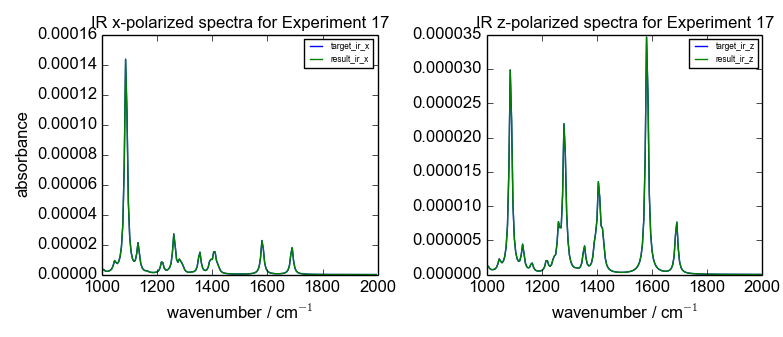
\includegraphics[scale=0.5]{Figures/chapter4_result_target_plotting_5datapoint_ir.png}
\caption{IR spectra plotted by using target composition and return composition of Case 17} \label{fig:4.2}
\end{figure}

\begin{figure}[!ht] 
\centering
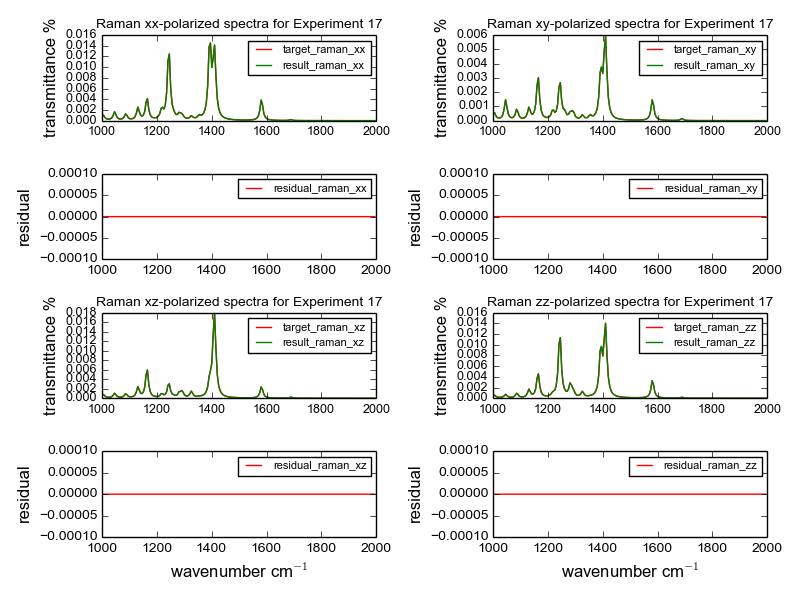
\includegraphics[scale=0.7]{Figures/chapter4_result_target_plotting_5datapoint_raman.png}
\caption{Raman spectra plotted by using the target composition and the return composition of Case 17} \label{fig:4.3}
\end{figure}

\begin{figure}[!ht]
\centering
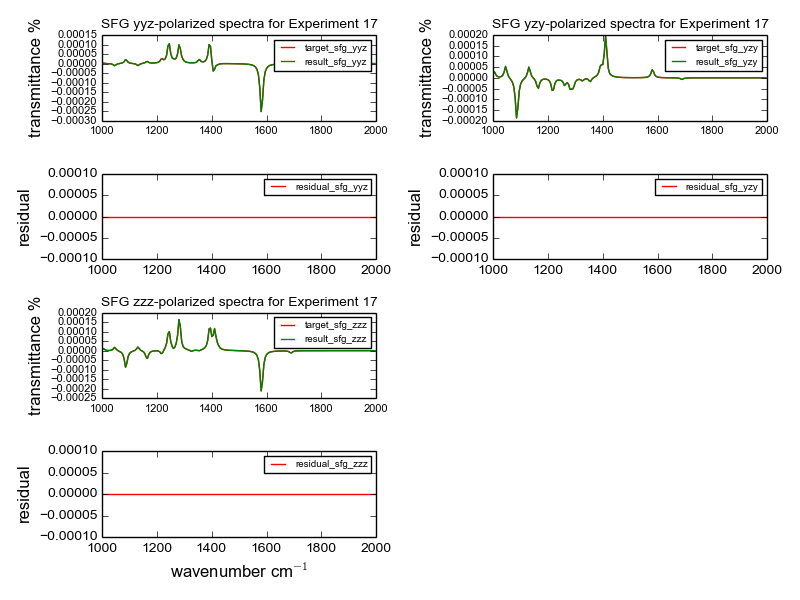
\includegraphics[scale=0.7]{Figures/chapter4_result_target_plotting_5datapoint_sfg.png}
\caption{SFG spectra plotted by using the target composition and the return composition of Case 17}  \label{fig:4.4}
\end{figure}

\begin{figure}[!ht] 
\centering
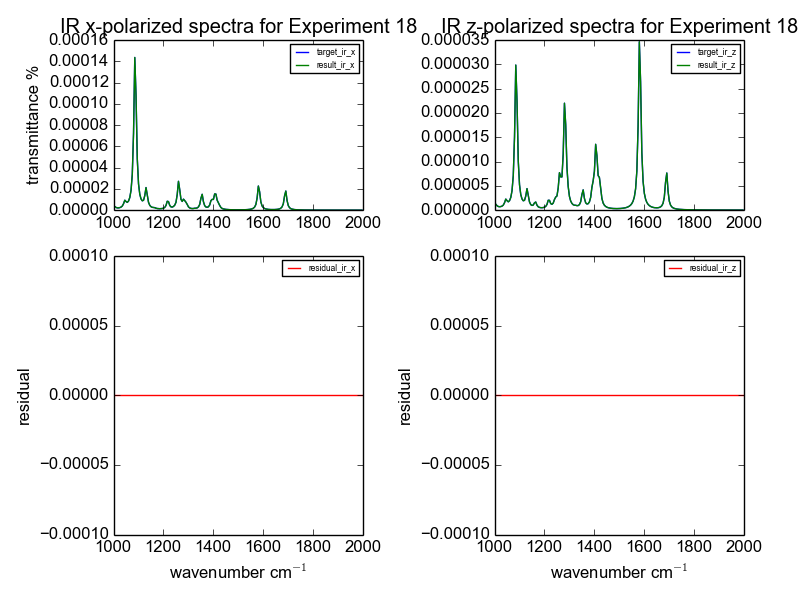
\includegraphics[scale=0.7]{Figures/chapter4_result_target_plotting_500datapoint_ir.png}
\caption{IR spectra plotted by using the target composition and the return composition of Case 18} \label{fig:4.5}
\end{figure}

\begin{figure}[!ht] 
\centering
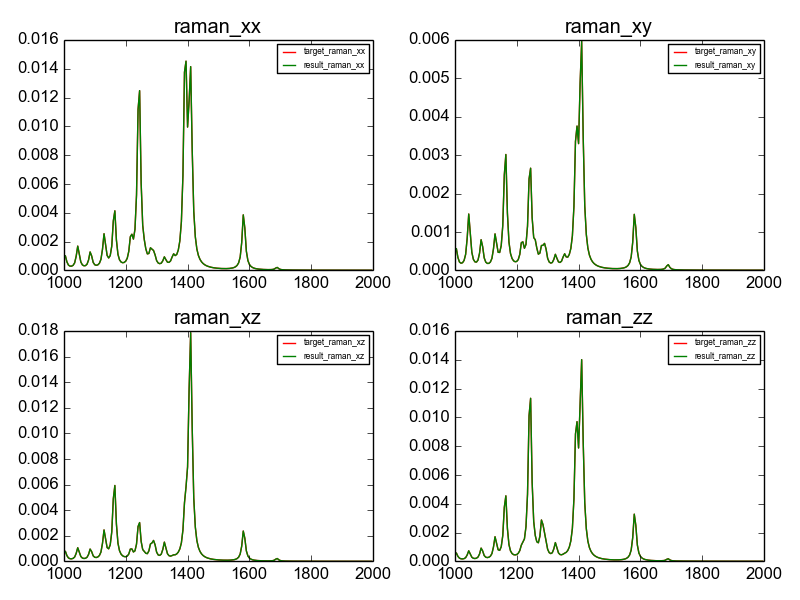
\includegraphics[scale=0.7]{Figures/chapter4_result_target_plotting_500datapoint_raman.png}
\caption{Raman spectra plotted by using the target composition and the return composition of Case 18} \label{fig:4.6}
\end{figure}

\begin{figure}[!ht] 
\centering
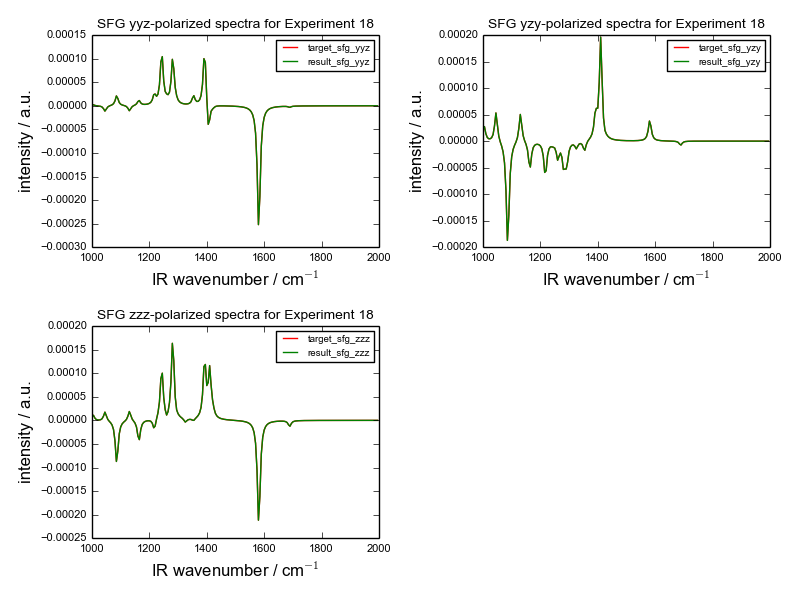
\includegraphics[scale=0.7]{Figures/chapter4_result_target_plotting_500datapoint_sfg.png}
\caption{SFG spectra plotted by using the target composition and the return composition of Case 18} \label{fig:4.7}
\end{figure} 

\section{Conclusion}



%\section{Extra Test Cases}
%TODO: this part of test cases are similar as what are done in Chapter 5 and 6. Think how to involve this part properly.

%From Case 1 to 18, LP model helps to return the target composition for some cases, and not for others. We want to figure out if there a clean line indicating the information used to generate the LP model is not sufficient to obtain the target composition for one molecule. In order to answer this question, more systematic test cases needed to be organized. Therefore, the following test cases are conducted. The Methionine candidate space is the same as Case 17 and 18. spread from $0^{\circ}$ to $80^{\circ}$ on $\theta$. 






	\startchapter{Mixture of Realistic Molecules} \label{ch:5}
\section{Description}

In Chapter \ref{ch:4}, test cases indicate that for one type of molecule at surfaces, even when combining the information of all the three spectral information, the built LP instances are still not sufficient to obtain the target composition in most test cases. In another word, the existing spectral information is not adequate to obtain the target composition of one type of molecule at surfaces. Multiple return compositions can build the target spectra. Besides one type of molecule at surfaces, we are also interested in the case where candidates coming from different molecules. For a mixture of different molecules at surfaces, we want to figure out with available spectral information, can the LP model help to return the target composition. In the case where the LP model is sufficient to compute the target composition, we are interested in which the specific combination of spectroscopy techniques is sufficient. Moreover, we want to know the accuracy of this specific combination in obtaining the target composition. \\

\section{Test Cases}
The first part of this section, we study the cases where each molecule's candidates expanded from $0^{\circ}$ to $80^{\circ}$ on $\theta$ to see which spectral information is sufficient in obtaining the target composition. Then in the second part, we study the cases where we study the cases where each molecule's candidates expanded from $0^{\circ}$ to $180^{\circ}$ on $\theta$. \\

\subsection{Test Cases Considering Each Amino Acid Candidates from $\theta$ $0^{\circ}$ to $80^{\circ}$ in the Mixture of Realistic Molecules} \label{testcase51}
To study the molecular orientation distribution of various molecules at surfaces, further test cases are constructed. These test cases have the following common settings. \\

First, as mentioned in Chapter \ref{ch:1}, there are six different amino acids in the mixture: Met, Leu, Ile, Ala, Thr and Val. For each amino acid, only the difference of $\theta$ is considered. Each amino acid has nine candidates in the mixture. They have the following $\theta$ values: $0^{\circ}$,  $10^{\circ}$, $20^{\circ}$, $30^{\circ}$, $40^{\circ}$, $50^{\circ}$, $60^{\circ}$, $70^{\circ}$ and $80^{\circ}$. When $\theta$ equals $90^{\circ}$, the SFG spectra has zero intensity. Therefore the corresponding candidate is excluded from all the test cases. As a result, there are 54 candidates in the mixture. \\

Second, the target composition needs to be generated. The operation includes two steps: randomly pick one candidate from each of the amino acid's nine candidates, then randomly generate a percentage for the selected candidate. The target composition is made of six randomly selected candidates with assigned percentage coming from the amino acids. The remaining $48$ candidates have $0$ percentage in the target composition. That is six selected candidate makes 100\% component of the mixture. \\

Third, the IR, Raman and SFG spectra need to be generated for all $54$ candidates and the target. \\

Table \ref{tab:5.1} displays a set of test cases. Each test case contains different spectral information. In Case 1, candidates $x$- and $z$-polarized IR spectra are obtained. The target's IR spectra are generated by the dot product of the target composition and all the candidates' spectral data. Then the corresponding LP instance is conducted using Equation \ref{eq:3.4}. Therefore, we conclude that in Case 1, only IR information is used to build the LP instance. Similarly, in Case 2, only Raman spectral information is used to build the LP instance. In Case 3, only SFG spectral information is used to build the LP instance. \\

\begin{table}[ht!]
\begin{center}
{\def\arraystretch{1.5}
\begin{tabular}{| l | p{3in} | }
\hline
Test Case & Spectral Information \\
\hline
Case 1 & $x$ and $z$ polarized IR spectra\\
\hline
Case 2 & $xx$, $xy$, $xz$ and $zz$ polarized Raman spectra \\
\hline
Case 3 & $xxz$, $xzx$ and $zzz$ polarized SFG spectra \\
\hline
Case 4 & $x$ and $z$ polarized IR spectra \newline $xx$, $xy$, $xz$ and $zz$ polarized Raman spectra \\
\hline
Case 5 & $x$ and $z$ polarized IR spectra \newline $xxz$, $xzx$ and $zzz$ polarized SFG spectra \\
\hline
Case 6 & $xx$, $xy$, $xz$ and $zz$ polarized Raman spectra \newline $xxz$, $xzx$ and $zzz$ polarized SFG spectra \\
\hline
Case 7 & $x$ and $z$ polarized IR spectra \newline
 $xx$, $xy$, $xz$ and $zz$ polarized Raman spectra \newline 
 $xx$, $xzx$ and $zzz$ polarized SFG spectra \\
\hline
\end{tabular} 
}
\end{center}
\caption{Detailed test cases set for the mixture of amino acids.} 
\label{tab:5.1} 
\end{table}	

Starting from Case 4, spectral information of different spectroscopy techniques are combined to build the LP instance. In Case 4, IR spectral information is combined with Raman. In Case 5, IR spectral information is combined with SFG. In Case 6, Raman and SFG spectral information are incorporated. At the end, in Case 7, information of all three spectral is put together: IR, Raman and SFG. \\

Finally, this set of test cases is run 100 times in order to see which test case in the set returns the target composition with the highest accuracy. This accuracy is measured by the time of the LP solver returns the target composition. The scoring mechanism that measures whether or not a return composition matches the target one is described in the next section. \\

\subsection{Scoring method}

At the first glance, it may appear a useful approach that the sum of residuals between the spectra composed by the return composition and the target one can be used to measure the accuracy of the return composition. However, recall that in most test cases conducted earlier, the spectra generated by the return composition are identical to the target ones. The sum of residuals between these spectra is negligible, which makes it appropriate to use it as a scoring criterion. \\

Another way to measure the accuracy of the return composition is to compare it directly with the target composition. Calculating the sum of the residuals between a target composition and a return one directly can be a fast approach to evaluate the accuracy of each test case. The shortage of this approach is that it cannot be used to measure in realistic test cases where the target composition is unknown. However, in the current test cases, this approach can be a way to evaluate the return composition for all the test cases where the target compositions are known in advance. \\

The return composition of each test case in the set is obtained for each run. Each return composition is compared with the target one to calculate the sum of the residuals. If the sum is smaller than a certain threshold, which is $10^{-7}$, then the return composition is considered to be the same as the target one. \\

\begin{figure}[!ht]
\centering
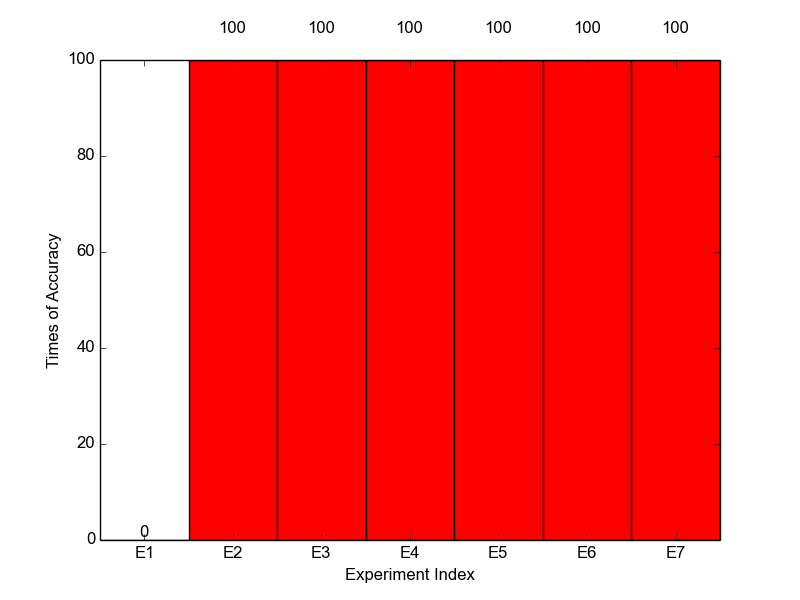
\includegraphics[scale=0.7]{Figures/accuracy_pecent_result8_mixture.png}
\caption{Accuracy analysis for test cases considering a mixture of amino acids with candidates from $0^{\circ}$ to $80^{\circ}$ on $\theta$ for each amino acid. Accuracy indicates how many times each test case in the set return a composition that matches the target one.}  \label{fig:5.1}
\end{figure}

The test case set is run 100 times, based on the scoring method, the result is shown in 
Figure \ref{fig:5.1}. Case 2, 3, 4, 5, 6 and 7 return the target composition in all 100 runs. This result indicates that Raman or SFG alone is sufficient to obtain the target composition, for a mixture of amino acids with candidates from $0^{\circ}$ to $80^{\circ}$ on $\theta$ for each amino acid. Any test cases that contain Raman and SFG spectral information result in the same accuracy. \\

The only exception is Case 1. The accuracy is fairly low, which indicates that IR spectra alone do not contain sufficient information in order to obtain the target composition. \\

To gain more understanding of the return composition of Case 1, the test case set is re-run 100 times. In each run, IR $x$- and $z$-polarized spectra are plotted both by the returned composition and the target one. The result is that these spectra conducted by the two different compositions are identical in each run. Let us randomly take one run as an example. Figure \ref{fig:5.2} displays the plotted spectra. Note that they are identical to each other. The residual is very small for the data points where these two spectra are not overlapped. This further indicates that IR spectral information is not sufficient to obtain the target composition.\\

%(TODO: rewrite or remove this paragraph) Comparatively, SFG has three unique polarizations, and Raman has four unique polarizations. From each projection's spectrum, we evenly select 200 data points. This means that one more projection will bring in 200 more constraints or 400 more (when we take the absolute sign off) constraints to the LP model. This would make a huge difference in the LP model, in term of further refining the candidate selection in target composition. However, it is still too early for us to say that Raman has more orientation information because it has four unique polarizations. Because for Raman's any polarization, the spectrum of candidate with $\theta$ equals to one degree is identical to the one of candidate with this $\theta$ degree's complementary. For example, the Raman spectra for candidate with $\theta$ of $10^{\circ}$, is the same as candidate with $\theta$ of $170^{\circ}$. And for IR, it is the same case. Only SFG tells the differences between these two degrees, as the spectra for candidate with $\theta$ of one degree is symmetric to its complementary along wavenumber as shown in Figure \ref{fig:5.8}. \\

\begin{figure}[!ht] 
\centering
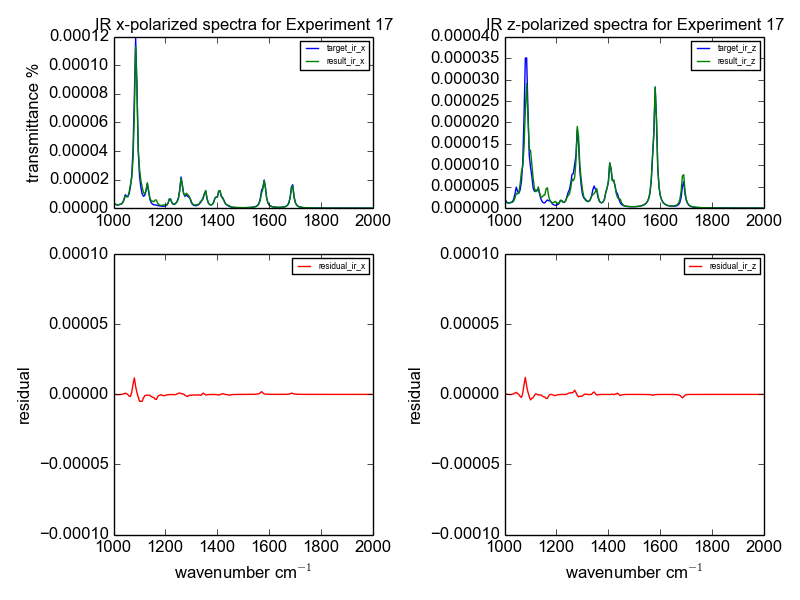
\includegraphics[scale=0.7]{Figures/chapter5_result_target_residual_plotting__ir_result8_run1.png}
\caption{IR spectra plotted by the result composition and the target composition of one ramdon run when considering each amino acid candidates from $0^{\circ}$ to $80^{\circ}$ on $\theta$ in the Mixture of realistic molecules.} \label{fig:5.2}
\end{figure}

\subsection{Test Cases Considering Each Amino Acid Candidates from $\theta$ $0^{\circ}$ to $180^{\circ}$ in the Mixture of Realistic Molecules}
To further study the capacity of the LP models, the candidate pool is expanded from $0^{\circ}$ to $180^{\circ}$ in terms of the $\theta$ value. Therefore, each amino acid has $18$ candidates. In total, there are $108$ candidates in the mixture. The same set of test cases as in Table \ref{tab:5.1} is used. The only difference is that instead of randomly selecting one candidate from nine candidates, it is selected from eighteen. All $108$ candidates' IR, Raman and SFG spectra need to be generated. Figure \ref{fig:5.3} illustrates the results obtained in $100$ runs. The accuracy in Case 1 is still low. This is not surprising as the complexity of the candidates has increased. Moreover, IR spectra for candidate of $\theta$ is identical to the one of $\theta$ complement, as shown in Figure \ref{fig:A.1}. This also increases the difficulty for the LP model to return the target composition. \\

\begin{figure}[!ht]
\centering
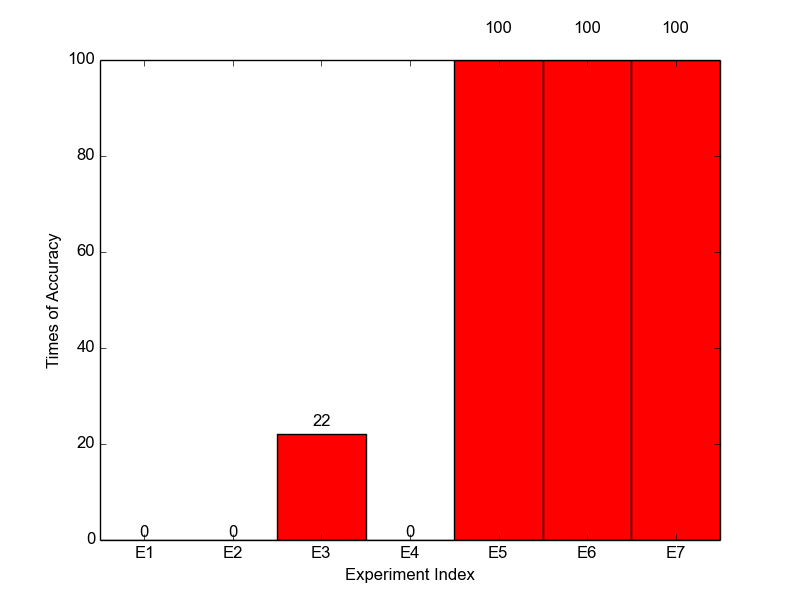
\includegraphics[scale=0.7]{Figures/accuracy_pecent_result10_mixture.png}
\caption{Accuracy analysis for test cases considering a mixture of amino acids with candidates from $0^{\circ}$ to $180^{\circ}$ on $\theta$ for each amino acid. Accuracy indicates how many times each test case in the set return a composition matches the target one.} \label{fig:5.3}
\end{figure}

However, it should be noted that the accuracy for Case 2 has dramatically dropped. This can be caused by the fact that the Raman spectra for one candidate with a $\theta$ is identical to the one of $\theta$ complement as displayed in Figure \ref{fig:A.2}. \\

Figure \ref{fig:5.3} shows that also the accuracy for Case 3 is no longer high. After increasing the number of amino acid candidates from nine to eighteen, the complexity of candidates has increased as well. SFG spectra from candidate of $\theta$ is symmetric to the one of $\theta$ complement, which has increased the difference of the candidates as shown in Figure \ref{fig:A.3}. However, the SFG spectral information is still not sufficient for obtaining the target composition. \\

The good result starts to emerge when using the combinations of IR and SFG or Raman and SFG. Figure \ref{fig:5.3} shows that Cases 5, 6, and 7 all have 100\% accuracies. SFG spectra is needed as it is the only information that distinguish $\theta$ from its complement. Once combining SFG spectral information with other technique to obtain extra spectral information, it is sufficient to obtain the target composition. \\

Although the accuracy in Case 2 is low, there is still some noticable result in the return composition: for each amino acid, the percentage assigned is correct; however, the candidate presented may not always be correct. We observe that it is either the correct $\theta$, or its complementary. We randomly select one run of the test case set as an example, Figure \ref{fig:5.4} displays the target composition. Figure \ref{fig:5.5} displays the return composition of Case 2. Figure \ref{fig:5.6} is the return composition of Case 6. Figure \ref{fig:5.4} and \ref{fig:5.6} are identical, which means the return composition of Case 6 is the same as the target one. The values in Figure \ref{fig:5.5} are the same as Figure \ref{fig:5.4}. However, the position of each value is not the same in two the figures. For example, the percentage value $0.30$ of Met is for $\theta = 120^{\circ}$ in Figure \ref{fig:5.4}, but is for $\theta = 60^{\circ}$ in Figure \ref{fig:5.5}. These two angles are complementary. This observation is the same for Ile, Ala, Thr, and Val in the figures. This observation is a general case across all the runs of the test case set. The return composition of Case 6 matches the target one. However, the return composition of Case 2 fails to pick the correct candidate of each amino acid from this candidate's $\theta$ complementary. This can be explained as the Raman spectra for a specific value of $\theta$ is the same as its complement. \\

\begin{figure}[!ht] 
\centering
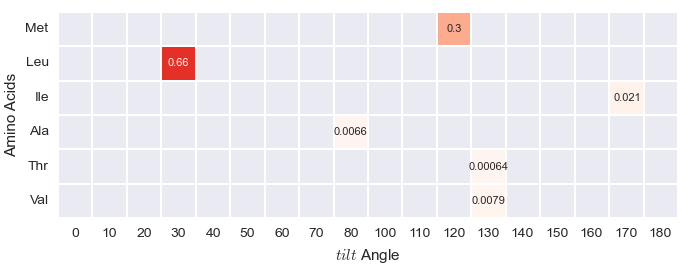
\includegraphics[scale=0.7]{Figures/mixture_target_composition_for_one_run_theta_0_180.png}
\caption{Target composition of one random run of six mixed amino acids with candidates expanded from $0^{\circ}$ to $180^{\circ}$ on $\theta$ for each amino acid. More detailed data of this target composition can be found in Appendix \ref{eqn:A.1}. } 
\label{fig:5.4}
\end{figure}

\begin{figure}[!ht] 
\centering
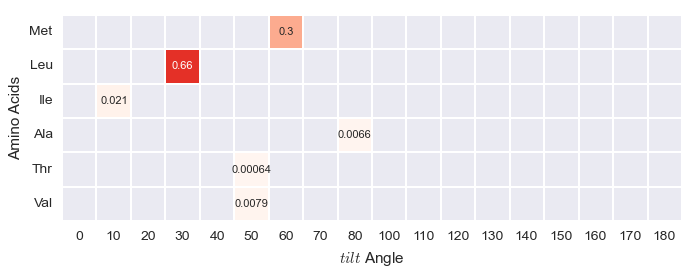
\includegraphics[scale=0.7]{Figures/mixture_return_composition_of_E2_for_one_run_theta_0_180.png}
\caption{Return composition of Case 2 for one random run of six mixed amino acids with candidates expanded from $0^{\circ}$ to $180^{\circ}$ on $\theta$. More detailed data of this return composition can be found in Appendix \ref{eqn:A.2}.} 
\label{fig:5.5}
\end{figure}

\begin{figure}[!ht] 
\centering
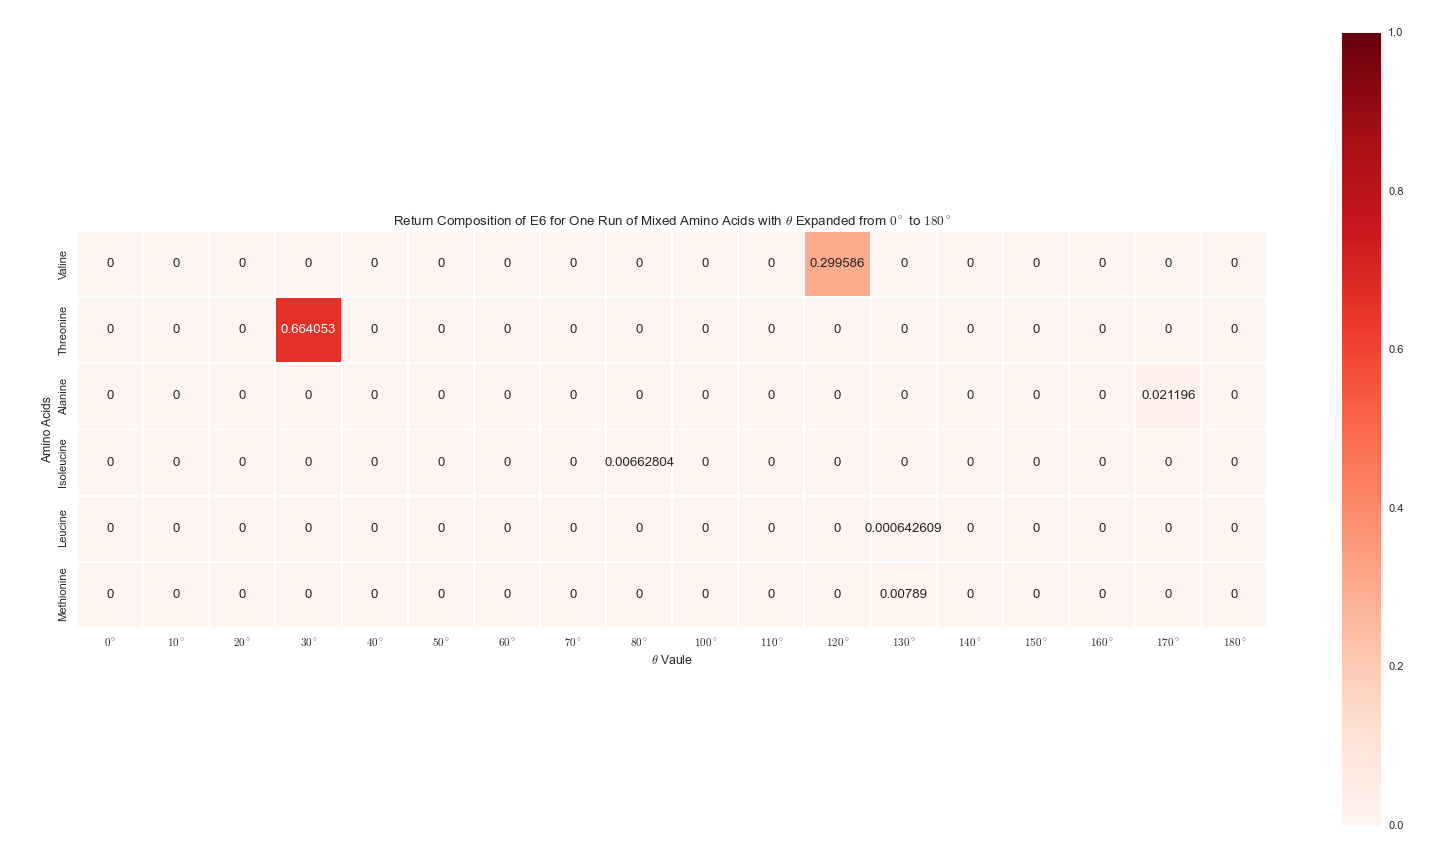
\includegraphics[scale=0.7]{Figures/mixture_return_composition_of_E6_for_one_run_theta_0_180.png}
\caption{Return composition of Case 6 for one random run of six mixed amino acids with candidates expanded from $0^{\circ}$ to $180^{\circ}$ on $\theta$. More detailed data of this return composition can be found in Appendix \ref{eqn:A.3}.} 
\label{fig:5.6}
\end{figure}

\section{Conclusion}
Raman and SFG spectral information each alone is sufficient to obtain the target composition, when considering a mixture of molecules with candidates expanded from $0^{\circ}$ to $80^{\circ}$ on $\theta$ for each amino acid. When the candidates of each molecule are expanded from $0^{\circ}$ to $180^{\circ}$ on $\theta$, SFG spectral information needs to be combined with IR or Raman in order to obtain the target composition. SFG spectral information is needed, as it is the only information to distinguish candidate of $\theta$ from its complement.\\

	\startchapter{Possibilities for treating experimental data} \label{ch:6}
\section{Description}
The experimental spectra obtained from IR, Raman or SFG techniques have an amplitude scaling factor when comparing to the candidate spectra generated mathematically. This means that between candidates' theoretical spectra and the experimental one, there is an unknown scaling factor. Within one particular spectroscopy technique, this scaling factor is the same for any polarization. Take IR as an example, the scaling factor for the spectrum of $x$ polarization is the same as the one for the spectrum of $z$ polarization. It is necessary to introduce this scaling factor to the LP models. The LP models constructed by Experiment 2 to 7 in Table \ref{tab:5.1} for $\theta$ ranged from $0^{\circ}$ to $80^{\circ}$) are doing well in retrieving the target composition for the mixed amino acids. Therefore, based on these experiments, we would like to know if the same LP models can be applied directly to the real experimental data for the same $\theta$ range.\\

Therefore, the same experiment setting in Table \ref{tab:5.1} are used for the following experiments. The goal is the same, to figure out which spectral information helps to retrieve the target composition for the mixture of six amino acids' candidates. The only difference is that, in each run of the experiment set, an arbitrary scaling factor is generated for IR, Raman and SFG, respectively. Therefore, the target spectra is not only composed by the target composition of all candidates, but also need to multiple by the randomly generated scaling factors of each spectroscopy technique. \\

To start with, we limit the scaling factors to be smaller than 1. \\

After a few runs of the experiment set, it is observed that the returned compositions always contains one extra variable in every experiment. For Experiment 2, 4, 6 and 7, the returned composition contains the right selected candidates. However, the percentage values of the candidates are different from the target composition. The ratio between the returned percentage and the target percentage are the same for the selected candidates. Furthermore, when this ratio adds up the extra variable, it equals $1$. Randomly select one experiment run, then take Experiment 2 as an example. Figure \ref{fig:6.2} displays the target composition generated, only the selected candidates are annotated with assigned percentage. Figure \ref{fig:6.2} displays the return composition of Experiment 2. The selected candidates in the return composition are in the right position, however, each percentage value is different from the one in the target composition. There are one extra value in Figure \ref{fig:6.2} whith value of $0.4$. \\

\begin{figure}[!ht] 
\centering
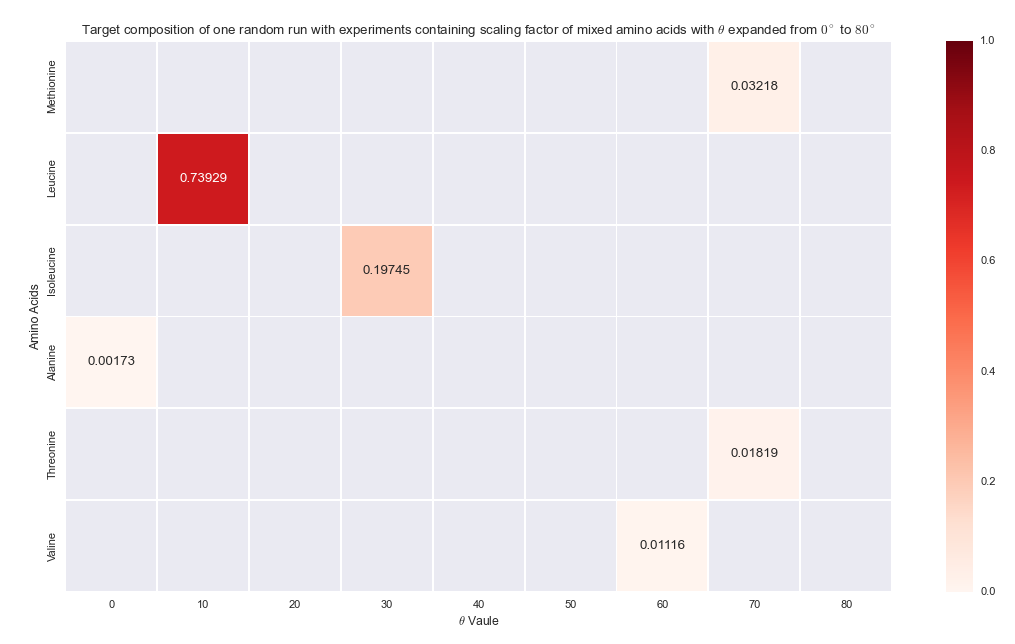
\includegraphics[scale=0.5]{Figures/chapter6_figure_one.png}
\caption{Target composition for one random run of experiment set with scaling foctor for mixed amino acids with $\theta$ expended from $0^{\circ}$ to $80^{\circ}$} \label{fig:6.1}
\end{figure}


\begin{figure}[!ht] 
\centering
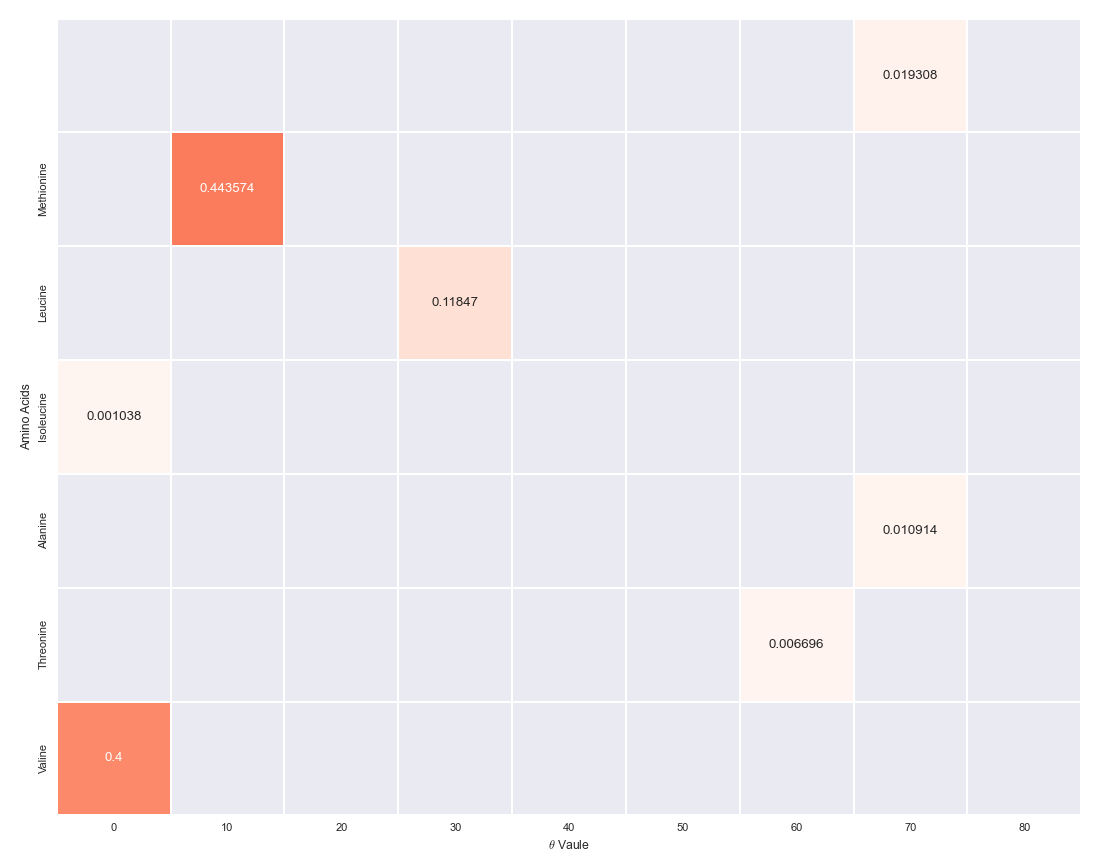
\includegraphics[scale=0.4]{Figures/chapter6_figure_two.png}
\caption{Return composition of Experiment 2 for one random run of experiment set with scaling foctor for mixed amino acids with $\theta$ expended from $0^{\circ}$ to $80^{\circ}$} \label{fig:6.2}
\end{figure}

Moreover, as Equation \ref{eqn:6.3} shows the ratio between the percentage of the selected candidates in the return composition and the target one is the same for all the amino acids. The value of this ratio is $0.6$. When this ratio is added up with the extra variable (referred as slack variable in LP) $0.4$, the total is $1$. As the scaling factors are pre-generated in the experiment set, the value is known, which is $0.6$. In conclusion, the slack variable (SV) is returned by LP. Then the scaling factor (SF) equals to $1 - SV$. From the scaling factor, the ratio between the return composition and the target one is known. At the end, the target composition can be re-built from the ratio and the return composition. The re-constructed target composition matches to the original one. \\

\begin{eqnarray} \label{eqn:6.3}
\frac{0.019308}{0.03218} = \frac{0.443574}{0.73929} = \frac{0.11847}{0.19745} =\frac{0.001038}{0.00173}  = \frac{0.010914}{0.01819} = \frac{0.006696}{0.01116} = 0.6
\end{eqnarray}

\begin{figure}[!ht] 
\centering
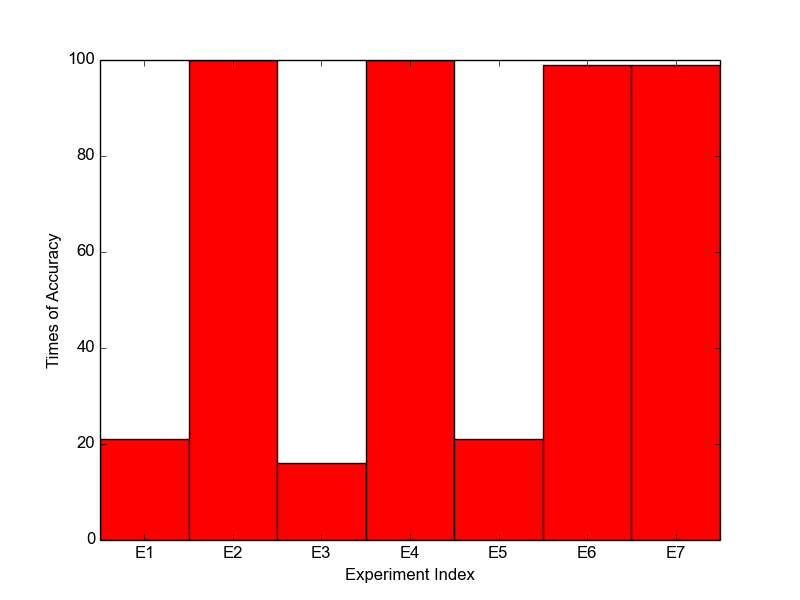
\includegraphics[scale=0.5]{Figures/chapter6_1.png}
\caption{Experiment Accuracy Analysis for Experiments using experimental spectra data that contains scaling factor that is smaller than 1 and candidates with $\theta$ from $0^{\circ}$ to $80^{\circ}$}
\label{fig:6.3}
\end{figure}

To check whether the above observation is a general case, the experiment set in Table \ref{tab:5.1} is run 100 times with randomly generated scaling factors in each run. Figure \ref{fig:6.3} indicates the experiment result. Figure \ref{fig:6.3} shows that Experiment 2, 4, 6 and 7 almost hit the above observation with $100%$ frequency. This indicates that even with the scaling factor, Raman spectral information alone is sufficient to study the mixed molecules' coordination distribution at interfaces. The target composition can be re-constructed correctly from the return slack variable and the return composition. Figure \ref{fig:6.3} also illustrates that Experiment 3, the LP model with only SFG spectral information, does not hit the above observation with high frequency. With the scaling factor as the addition, SFG spectral information is not sufficient to obtain the target composition. Even combining IR and SFG spectral information, the constructed LP model cannot help to re-construct the target composition. \\

The return slack variable and composition of Experiment 4, 6 and 7 are the same as Experiment 2 in each run. This indicates Raman spectral information are dominating the solution in the LP model. \\

%When the scaling factor is greater than 1, all LP models built by the 7 experiments will fail to obtain the correct composition of target spectrum. (TODO: check with Ulrike and Dennis to see if I need to include this part in my thesis.)\\

When each amino acid's candidates are expanded from $0^{\circ}$ to $180^{\circ}$ on $\theta$, the same experiment set is applied 100 times with randomly generated scaling factors in each run. The result in Figure \ref{fig:6.4} illustrates that none of the experiment in the set meets the observation with high frequency. \\

When the return compositions of Experiment 2 and 6 are further analyzed, there are few observation need to be noticed. To facilitate the explanation, one random run is picked as an explicit example. Figure \ref{fig:6.5} is the target composition. Figure \ref{fig:6.6} is the return composition of Experiment 2. Figure \ref{fig:6.7} is the return composition of Experiment 6. In Figure \ref{fig:6.6}, the slack variable still equals $1 - generated~scaling~factor$. For each amino acid, the selected candidate in the return composition may not be the exact one as the target composition selected. However, this selected candidate is always either the correct one in the target composition, or the correct one's $\theta$ complimentary. In Figure \ref{fig:6.7}, for each amino acid, there are two selected candidates in the return composition. These two selected candidates are the correct one and its $\theta$ complimentary. When the percentages of these two selected candidates are added, it is equalled to the percentage returned for the amino acid in Figure \ref{fig:6.7}. $0.0776716 + 0.0252641 = 0.102936$. Between these two selected candidates, the correct one's percentage is always bigger than its $\theta$ complimentary. $0.0776716 > 0.0252641$. In conclusion, Experiment 2 achieves in telling the slack variable, the scaling factor, and the ratio between the 

The LP model with only Raman spectral information Experiment 2, is able to tell us for each amino acid, candidate with which $\theta$ or this $\theta$'s complementary would exist in our target spectra. Because Raman spectra for candidate with $\theta$ on one degree is the same as its supplementary. This LP model can not distinguish between candidate with $\theta$ and the one with its complementary.However, with the help of SFG, we may be able to know which one between the above two dominates one amino acid's the total fraction, like what we have learnt from Chapter \ref{ch:5} about E6. Therefore we exam E6 here, and it displays which one of the two takes the major composition in the target spectra. With this information, we can decide between the $\theta$ and its complementary. 
With the information coming from E2 and E6, we therefore, obtain the right composition of the target spectrum.\\

Here goes the example, in one run of the experiment group. The composition for the target spectrum is Array \ref{eqn:6.4}. %($result8.txt of result_2016_09_28$)
In this target spectrum, we have 0.14799 of $\theta = 40^{\circ}$ Methionine, 0.74202 of $\theta = 50^{\circ}$ Leucine, 0.08989 of $\theta = 150^{\circ}$ Ile, 0.01135 of $\theta = 40^{\circ}$ Ala, 0.00715 of $\theta = 0^{\circ}$ Thr, 0.0016 of $\theta = 20^{\circ}$ Val. 

\begin{eqnarray}\label{eqn:6.4} 
\resizebox{\linewidth}{!}{$
\begin{bmatrix}
0& 0& 0& 0& 0.14799& 0& 0& 0& 0& 0& 0& 0& 0& 0& 0& 0& 0& 0\\
0& 0& 0& 0& 0& 0.74202& 0& 0& 0& 0& 0& 0& 0& 0& 0& 0& 0& 0\\
0& 0& 0& 0& 0& 0& 0& 0& 0& 0& 0& 0& 0& 0& 0.08989& 0& 0& 0\\
0& 0& 0& 0& 0.01135& 0& 0& 0& 0& 0& 0& 0& 0& 0& 0& 0& 0& 0\\
0.00715& 0& 0& 0& 0& 0& 0& 0& 0& 0& 0& 0& 0& 0& 0& 0& 0& 0\\
0& 0& 0.0016& 0& 0& 0& 0& 0& 0& 0& 0& 0& 0& 0& 0& 0& 0& 0
\end{bmatrix}
$}
\end{eqnarray}

\begin{eqnarray}\label{eqn:6.5} 
\resizebox{\linewidth}{!}{$
\begin{bmatrix}
0& 0& 0& 0& 0.102936& 0& 0& 0& 0& 0& 0& 0& 0& 0& 0& 0& 0& 0\\
0& 0& 0& 0& 0& 0.516118& 0& 0& 0& 0& 0& 0& 0& 0& 0& 0& 0& 0\\
0& 0& 0& 0.0625238& 0& 0& 0& 0& 0& 0& 0& 0& 0& 0& 0& 0& 0& 0\\
0& 0& 0& 0& 0.0078945& 0& 0& 0& 0& 0& 0& 0& 0& 0& 0& 0& 0& 0\\
0.00497324& 0& 0& 0& 0& 0& 0& 0& 0& 0& 0& 0& 0& 0& 0& 0& 0& 0\\
0& 0& 0.00111289& 0& 0& 0& 0& 0& 0& 0& 0& 0& 0& 0& 0& 0& 0& 0\\
0.304441
\end{bmatrix}
$}
\end{eqnarray}
The result returned by E2 is shown in Array \ref{eqn:6.5}. You may notice same as Array \ref{eqn:6.2} to Array \ref{eqn:6.1}, Array \ref{eqn:6.5} contains one more value than Array \ref{eqn:6.4}, 0.304441, which is the slack variable. We already know that the scaling factor is 0.695560510845(generated randomly, but recorded). When we add the slack variable and the scaling factor, the total comes up to 1.0. \\

In Array \ref{eqn:6.5}, we get 0.102936 of $\theta = 40^{\circ}$ Methionine, 0.516118 of $\theta = 50^{\circ}$ Leucine, 0.0625238 of $\theta = 30^{\circ}$ Ile, 0.0078945 of $\theta = 40^{\circ}$ Ala, 0.00497324 of $\theta = 0^{\circ}$ Thr, 0.00111289 of $\theta = 20^{\circ}$ Val. From Array \ref{eqn:6.6}, we can also deduce the value for the scaling factor.

\begin{eqnarray} \label{eqn:6.6}
\begin{split}
\frac{0.102936}{0.14799} &= \frac{0.516118}{0.74202} = \frac{0.0625238}{0.08989}  =\frac{0.0078945}{0.01135}  
\\
\\
&= \frac{0.00497324}{0.00715} = \frac{0.00111289}{0.0016} = 0.695560
\end{split}
\end{eqnarray}


At first glance, we may guess that this LP model actually return the correct composition. However, not all amino acids' composition is correct. For Ile, it should be 0.0625238 of $\theta = 150^{\circ}$, but the result returned 0.0625238 of $\theta = 30^{\circ}$, which is the complimentary of $150^{\circ}$. It is because these two degrees' Raman spectra are identical, there is no way for current LP model to distinguish these two. \\

With this information, we know the only thing we need to make sure is: is the $\theta$ returned by LP model the exact one in target spectrum or its complementary? (The above conclusion can also be applied to the experiments in Chapter \ref{ch:5} without the scaling factor. The LP model with only Raman spectra information can help us to see which $\theta$ of candidate and its complimentary should be for each amino acid. I did not observe this before.)\\

To answer this question, we need the help of SFG data. Because only SFG can tell us the difference between one angle and its complementary, as their spectra are symmetry, not identical around the axis of wevenumber.\\

In this experiment group, the result returned E6 is Array \ref{eqn:6.7}  (Second example???)
\begin{eqnarray}\label{eqn:6.7} 
\resizebox{\linewidth}{!}{$
\begin{bmatrix}
0& 0& 0& 0& 0.0776716& 0& 0& 0& 0& 0& 0& 0& 0& 0.0252641& 0& 0& 0& 0     \\
0& 0& 0& 0& 0& 0.3894440& 0& 0& 0& 0& 0& 0& 0.1266740& 0& 0& 0& 0& 0     \\
0& 0& 0& 0.0153456& 0& 0& 0& 0& 0& 0& 0& 0& 0& 0& 0.0471782& 0& 0& 0     \\
0& 0& 0& 0& 0.00595697& 0& 0& 0& 0& 0& 0& 0& 0& 0.00193762& 0& 0& 0& 0   \\
0.0037526& 0& 0& 0& 0& 0& 0& 0& 0& 0& 0& 0& 0& 0& 0& 0& 0& 0.00122061    \\
0& 0& 0.000839749& 0& 0& 0& 0& 0& 0& 0& 0& 0& 0& 0& 0& 0.000273144& 0& 0 \\
0.304441 (any relation for the fraction???)
\end{bmatrix}
$}
\end{eqnarray}

The value of the slack variable is the same as what returned by E2. However, the returned composition is totally different than what returned by E2. The interesting thing is that for each amino acid, the return existing candidates are complementary on $\theta$. The total percentage of these two candidates, take Methionine as an instance, $0.0776716 + 0.0252641$ makes 0.1029357 which is the same as what is returned by E2. This is the same for every amino acid. What's more, the composition returned by the E6 indicates which $\theta$ dominates the composition for one amino acid. For Methionine, $\theta = 40^{\circ}$ takes major part; for Leucine, $\theta = 50^{\circ}$ does; for Ile, $\theta = 30^{\circ}$ does; for Ala, $\theta = 40^{\circ}$ does; for Thr, $\theta = 0^{\circ}$  does; for Val, $\theta = 20^{\circ}$ does; And those candidates are the correct components for target spectra. 




IR+SFG, can you do anything with it???




\section{Results}
\section{Discussion}
\section{Conclusions}
\label{experimental}



	\startchapter{Conclusion and Future Work}  \label{ch:7}

\section{Conclusion}
In addition to existing two common approaches in studying the possible composition of candidates of model spectra, the use of LP has been explored by Hung \cite{KuoKaiHung:Thesis:2015}. It has been shown that LP can solve this problem in pseudo polynomial time $O(n)$, which is much better in computational gain than the traditionally exhaustive way of extracting molecular orientation information. However, the reason why the LP model does not always return the target composition of mock spectra was unknown. The first goal of this study is to figure out this reason. \\

The achieve the first goal, a simplified molecular model is designed to analyze the nature of the LP model. It has shown that as long as there is the right data set, the target composition is obtained. If the target composition is not returned correctly, then there is not sufficient spectral information to describe the test cases to the LP model. \\

Furthermore, when we use all the spectral information of a realistic molecule (Met) to build the LP instances, it is not guaranteed to return the target composition all the time. The spectral information we collect is not sufficient in describing the test cases to the LP model most of the time. \\

%With a detailed analysis of applying toy model IR spectral information to our LP model, we have learnt that the reason why our LP model does not return the target composition is that: the spectral data we extract does not always contain sufficient information in order for the LP model to converge to the target composition. As long as the data we collect is sufficient, the LP model guarantees to return a composition we expect. \\

%Based on this observation, we explore various cases. First of all, the case with candidates coming from type of molecule at interface is studied. In this case, the LP model cannot return a composition that match the target one most of the time. It is proved that is because the spectral data applied to the LP model does not contain sufficient information to obtain the target composition. \\

Following the scenario of having one type of realistic molecule at surfaces, the test cases of having multiple types of realistic molecules at surface are also explored. When each molecule's candidates expanded in $[0^{\circ}$, $90^{\circ})$ on $\theta$, Raman or SFG spectral information alone is sufficient to obtain the target composition. When the candidates are expanded in $[0^{\circ}$, $180^{\circ}]$ on $\theta$, SFG spectral information needs to combine with IR or Raman in order to obtain the target composition. \\

At last, instead of generating the target spectra by combining different candidates directly, they are obtained from real experimental data. Therefore, for each spectroscopy technique, there is a scaling factor between the candidate spectra generated theoretically and the real experimental target spectra. When consider a mixture of realistic molecules with candidates expanded in $[0^{\circ}$, $90^{\circ})$ on $\theta$, Raman spectral information alone is sufficient to obtain the target composition. Because the target composition can be re-constructed from the return SV and composition. The SF equals 1 minus SV. When each realistic molecule's candidates are expanded in $[0^{\circ}$, $180^{\circ}]$, both return compositions of using only Raman spectral information and using Raman and SFG spectral information are needed to obtain the target composition. \\

\section{Contributions}
\begin{itemize}
  \item By studying the LP instances built by using spectral information of simplified molecular model, lack of sufficient spectral information int the instances is the reason that the LP solver does not return the target composition in some test cases.
  \item In the case of studying one type of realistic molecular model at surfaces, even combining all three spectral information of IR, Raman and SFG to build the LP instances, it is not sufficient to obtain the target composition for most test cases. 
  \item In the case of different types of realistic molecular models at surfaces, Raman or SFG spectral information alone is sufficient to obtain the target composition when candidates of each molecular model expanded in $[0^{\circ}$, $90^{\circ})$ on $\theta$ value. When candidates of each molecular model expanded in $[0^{\circ}$, $180^{\circ}]$ on $\theta$ value, SFG spectral information needs to be combined with IR or Raman to obtain the target composition.
  \item When the slack variable is introduced to each spectral technique, the case of different types of realistic molecular models at surfaces is considered. When each molecular model's candidates expanded in $[0^{\circ}$, $90^{\circ})$ on $\theta$ value, Raman spectral information alone is sufficient to obtain the target composition. When each molecular model's candidates expanded in $[0^{\circ}$, $180^{\circ}]$ on $\theta$ value, the return compositions, of the LP instances using only Raman spectral information and using Raman and SFG spectral information, are both needed to obtain the target composition.
\end{itemize}

\section{Future Work}
Our LP model has proven its efficiency in studying molecular orientation distribution at surfaces when different molecules are considered. However, when considering one type of molecule at the surface, there is not enough spectral information for the LP model to obtain the target composition. One of the most important direction is to collect more spectral information to the LP model. Another direction is to combine LP technique with other computation model to further constraint the solution space of the target composition.









	\appendix
	\startappendix{Additional Information}
\label{chapter:appendix}
Detailed data value for Figure \ref{fig:5.4}
\begin{eqnarray} 
\resizebox{0.9\linewidth}{!}{$
\begin{bmatrix}
0& 0& 0& 0& 0& 0& 0& 0& 0& 0& 0& 0.299586& 0& 0& 0& 0& 0& 0\\
0& 0& 0& 0.664053& 0& 0& 0& 0& 0& 0& 0& 0& 0& 0& 0& 0& 0& 0\\
0& 0& 0& 0& 0& 0& 0& 0& 0& 0& 0& 0& 0& 0& 0& 0& 0.021196& 0\\
0& 0& 0& 0& 0& 0& 0& 0& 0.00662804& 0& 0& 0& 0& 0& 0& 0& 0& 0\\
0& 0& 0& 0& 0& 0& 0& 0& 0& 0& 0& 0& 0.000642609& 0& 0& 0& 0& 0\\
0& 0& 0& 0& 0& 0& 0& 0& 0& 0& 0& 0& 0.00789& 0& 0& 0& 0& 0
\end{bmatrix}
$}
\label{eqn:A.1}
\end{eqnarray}

Detailed data value for Figure \ref{fig:5.5}
\begin{eqnarray}
\resizebox{0.9\linewidth}{!}{$
\begin{bmatrix}
0& 0& 0& 0& 0& 0& 0.299586& 0& 0& 0& 0& 0& 0& 0& 0& 0& 0& 0\\
0& 0& 0& 0.664053& 0& 0& 0& 0& 0& 0& 0& 0& 0& 0& 0& 0& 0& 0\\
0& 0.021196& 0& 0& 0& 0& 0& 0& 0& 0& 0& 0& 0& 0& 0& 0& 0& 0\\
0& 0& 0& 0& 0& 0& 0& 0& 0.00662804& 0& 0& 0& 0& 0& 0& 0& 0& 0\\
0& 0& 0& 0& 0& 0.000642609& 0& 0& 0& 0& 0& 0& 0& 0& 0& 0& 0& 0\\
0& 0& 0& 0& 0& 0.00789& 0& 0& 0& 0& 0& 0& 0& 0& 0& 0& 0& 0
\end{bmatrix}
$}
\label{eqn:A.2}
\end{eqnarray}

Detailed data value for Figure \ref{fig:5.6}
\begin{eqnarray}
\resizebox{0.9\linewidth}{!}{$
\begin{bmatrix}
0& 0& 0& 0& 0& 0& 0& 0& 0& 0& 0& 0.299586& 0& 0& 0& 0& 0& 0\\
0& 0& 0& 0.664053& 0& 0& 0& 0& 0& 0& 0& 0& 0& 0& 0& 0& 0& 0\\
0& 0& 0& 0& 0& 0& 0& 0& 0& 0& 0& 0& 0& 0& 0& 0& 0.021196& 0\\
0& 0& 0& 0& 0& 0& 0& 0& 0.00662804& 0& 0& 0& 0& 0& 0& 0& 0& 0\\
0& 0& 0& 0& 0& 0& 0& 0& 0& 0& 0& 0& 0.000642609& 0& 0& 0& 0& 0\\
0& 0& 0& 0& 0& 0& 0& 0& 0& 0& 0& 0& 0.00789& 0& 0& 0& 0& 0
\end{bmatrix}
$}
\label{eqn:A.3}
\end{eqnarray}


Detailed data value for Figure \ref{fig:6.1}
\begin{eqnarray}
\resizebox{0.5\linewidth}{!}{$
\begin {bmatrix}
0& 0& 0& 0& 0& 0& 0& 0.03218& 0 \\
0& 0.73929& 0& 0& 0& 0& 0& 0& 0 \\
0& 0& 0& 0.19745& 0& 0& 0& 0& 0 \\
0.00173& 0& 0& 0& 0& 0& 0& 0& 0 \\
0& 0& 0& 0& 0& 0& 0& 0.01819& 0 \\ 
0& 0& 0& 0& 0& 0& 0.01116& 0& 0
\end {bmatrix} 
$}
\label{eqn:A.4}
\end{eqnarray}

Detailed data value for Figure \ref{fig:6.2}
\begin{eqnarray}
\resizebox{0.5\linewidth}{!}{$
\begin {bmatrix}
0& 0& 0& 0& 0& 0& 0& 0.019308& 0 \\
0& 0.443574& 0& 0& 0& 0& 0& 0& 0 \\
0& 0& 0& 0.11847& 0& 0& 0& 0& 0  \\
0.001038& 0& 0& 0& 0& 0& 0& 0& 0 \\ 
0& 0& 0& 0& 0& 0& 0& 0.010914& 0 \\
0& 0& 0& 0& 0& 0& 0.006696& 0& 0 \\
0.4
\end {bmatrix}
$}
\label{eqn:A.5}
\end{eqnarray}

Detailed data value for Figure \ref{fig:6.4}. Target composition
\begin{eqnarray}
\resizebox{0.9\linewidth}{!}{$
\begin {bmatrix}
& 0& 0& 0& 0& 0.53762& 0& 0& 0& 0& 0& 0& 0& 0& 0& 0& 0& 0 \\
0& 0& 0.26894& 0& 0& 0& 0& 0& 0& 0& 0& 0& 0& 0& 0& 0& 0& 0 \\
0& 0& 0& 0& 0& 0& 0& 0& 0& 0& 0.03951& 0& 0& 0& 0& 0& 0& 0 \\
0& 0& 0& 0& 0& 0& 0& 0& 0& 0& 0& 0& 0& 0& 0& 0.11382& 0& 0 \\ 
0& 0& 0& 0& 0.01604& 0& 0& 0& 0& 0& 0& 0& 0& 0& 0& 0& 0& 0 \\
0& 0& 0.02407& 0& 0& 0& 0& 0& 0& 0& 0& 0& 0& 0& 0& 0& 0& 0 \\
\end {bmatrix}
$}
\label{eqn:A.6}
\end{eqnarray}

Detailed data value for Figure \ref{fig:6.5}. Return composition of Result 2
\begin{eqnarray}
\resizebox{0.9\linewidth}{!}{$
\begin {bmatrix}
0& 0& 0& 0& 0& 0.414239& 0& 0& 0& 0& 0& 0& 0& 0& 0& 0& 0& 0 \\
0& 0& 0.20722& 0& 0& 0& 0& 0& 0& 0& 0& 0& 0& 0& 0& 0& 0& 0 \\ 
0& 0& 0& 0& 0& 0& 0& 0.0304427& 0& 0& 0& 0& 0& 0& 0& 0& 0& 0 \\
0& 0& 0.0876989& 0& 0& 0& 0& 0& 0& 0& 0& 0& 0& 0& 0& 0& 0& 0 \\
0& 0& 0& 0& 0.0123589& 0& 0& 0& 0& 0& 0& 0& 0& 0& 0& 0& 0& 0 \\
0& 0& 0.0185461& 0& 0& 0& 0& 0& 0& 0& 0& 0& 0& 0& 0& 0& 0& 0 \\
0.229495& 0& 0& 0& 0& 0& 0& 0& 0& 0& 0& 0& 0& 0& 0& 0& 0& 0 \\
\end {bmatrix}
$}
\label{eqn:A.7}
\end{eqnarray}

Detailed data value for Figure \ref{fig:6.6}. Return composition of Result 6
\begin{eqnarray}
\resizebox{0.9\linewidth}{!}{$
\begin {bmatrix}
0& 0& 0& 0& 0& 0.27162& 0& 0& 0& 0& 0& 0& 0.142619& 0& 0& 0& 0& 0 \\
0& 0& 0.135875& 0& 0& 0& 0& 0& 0& 0& 0& 0& 0& 0& 0& 0.0713442& 0& 0 \\ 
0& 0& 0& 0& 0& 0& 0& 0.0104812& 0& 0& 0.0199615& 0& 0& 0& 0& 0& 0& 0 \\
0& 0& 0.0301941& 0& 0& 0& 0& 0& 0& 0& 0& 0& 0& 0& 0& 0.0575048& 0& 0 \\
0& 0& 0& 0& 0.00810383& 0& 0& 0& 0& 0& 0& 0& 0& 0.00425508& 0& 0& 0& 0 \\
0& 0& 0.0121608& 0& 0& 0& 0& 0& 0& 0& 0& 0& 0& 0& 0& 0.00638527& 0& 0 \\ 
0.229495& 0& 0& 0& 0& 0& 0& 0& 0& 0& 0& 0& 0&0& 0& 0& 0& 0 \\
\end {bmatrix}
$}
\label{eqn:A.8}
\end{eqnarray}
%$g1 0.863411197459 g2 0.770505232571 g3 0.239946797277$

\begin{eqnarray} 
\resizebox{0.9\linewidth}{!}{$
\frac{0.019308}{0.03218} = \frac{0.443574}{0.73929} = \frac{0.11847}{0.19745} =\frac{0.001038}{0.00173}  = \frac{0.010914}{0.01819} = \frac{0.006696}{0.01116} = 0.6
$} \label{eqn:A.9}
\end{eqnarray}

\begin{eqnarray} 
\resizebox{0.9\linewidth}{!}{$
\begin{split}
\frac{0.414239}{0.53762} &= \frac{0.20722}{0.26894} = \frac{0.0304427}{0.03951}  =\frac{0.0876989}{0.11382} = \frac{0.0123589}{0.01604} = \frac{0.0185461}{0.02407} = 0.770505
\end{split}
$}\label{eqn:A.10}
\end{eqnarray}


\begin{figure}[!ht] 
\centering
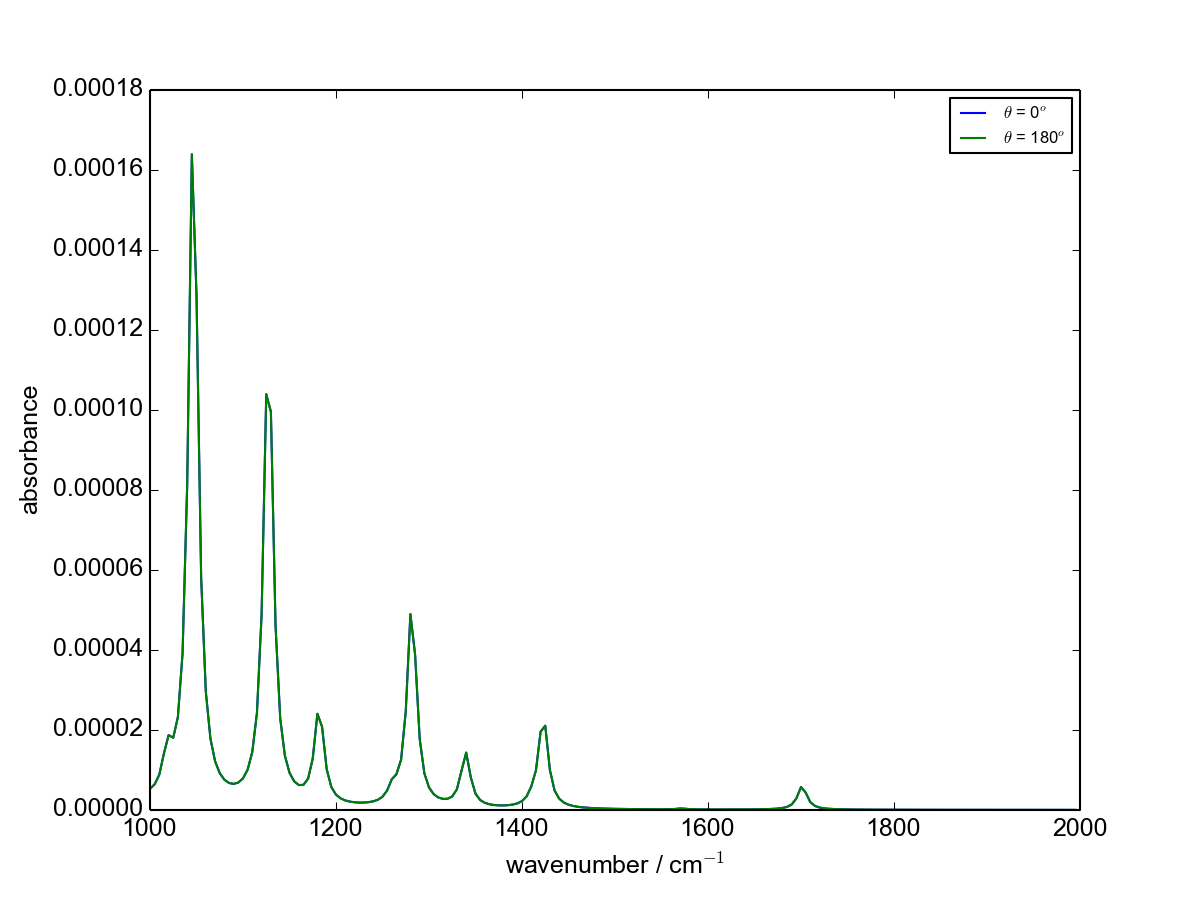
\includegraphics[scale=0.7]{Figures/Ala_candidates_plotting_ir_z_2.png}
\caption{IR $z$ projection spectrum for alanine candidate with $\theta$ of $0^{\circ}$ is identical to alanine candidate with $\theta$ of $180^{\circ}$.} \label{fig:A.1}
\end{figure}

\begin{figure}[!ht] 
\centering
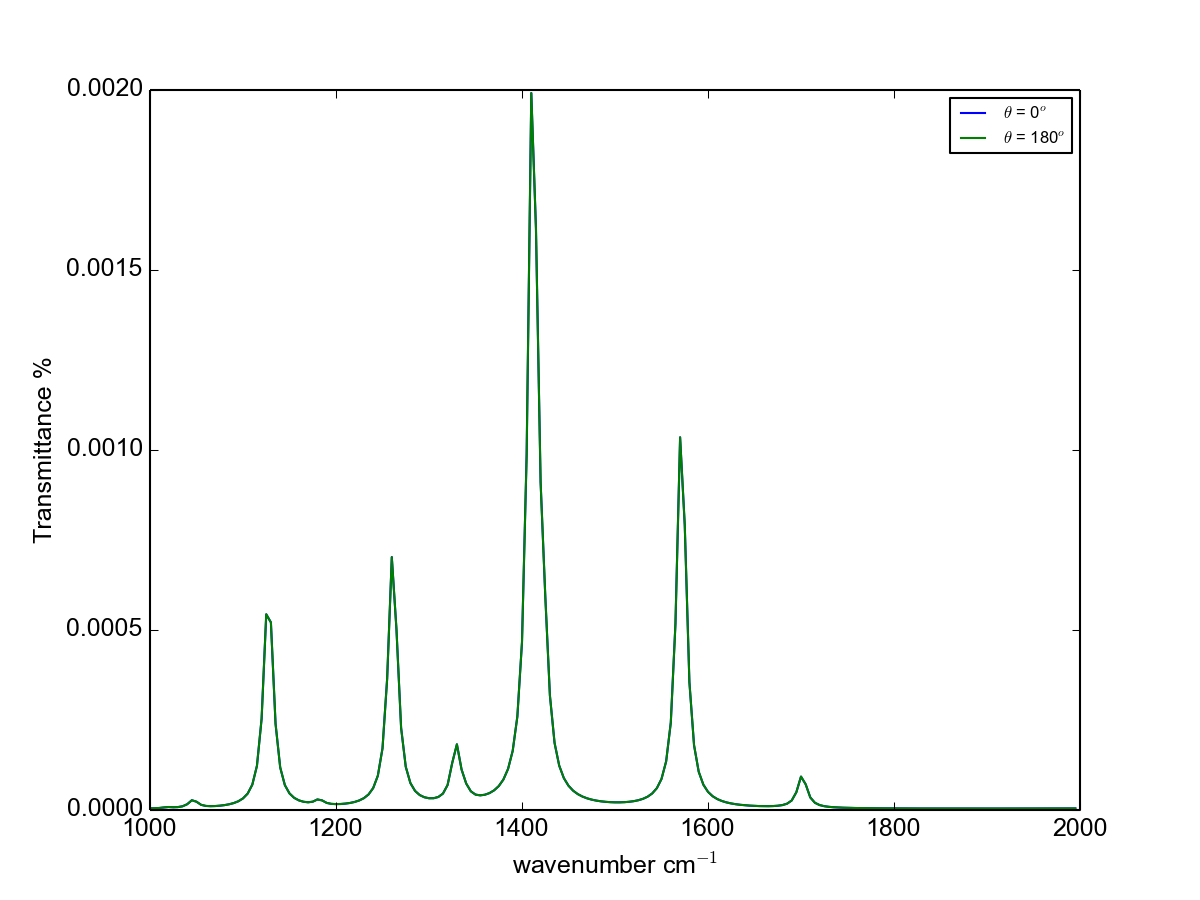
\includegraphics[scale=0.7]{Figures/Ala_candidates_plotting_raman_zz_2.png}
\caption{Raman $zz$ projection spectrum for alanine candidate with $\theta$ of $0^{\circ}$ is identical to alanine candidate with $\theta$ of $180^{\circ}$.} \label{fig:A.2}
\end{figure}

\begin{figure}[!ht] 
\centering
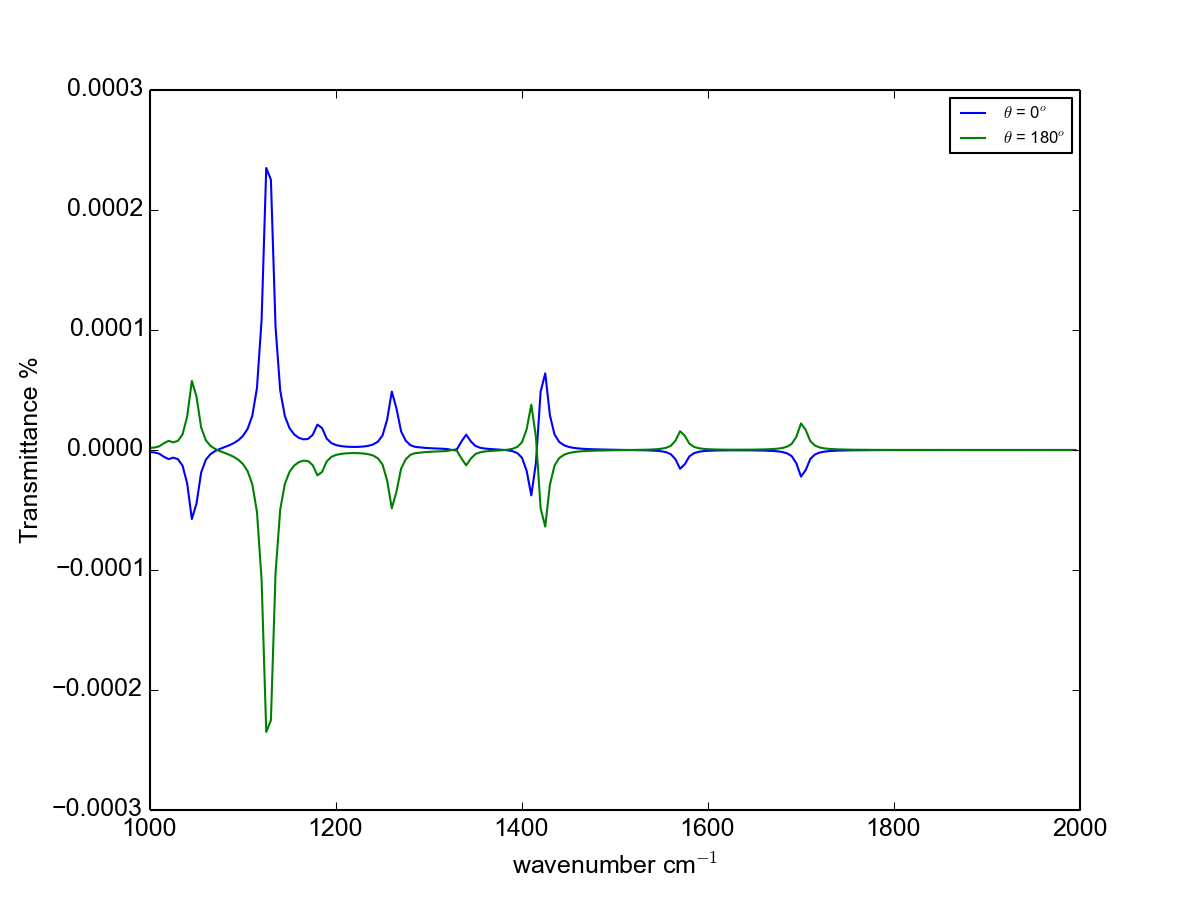
\includegraphics[scale=0.7]{Figures/Ala_candidates_plotting_sfg_zzz_2.png}
\caption{SFG $zzz$ projection spectrum for alanine candidate with $\theta$ of $0^{\circ}$ is not identical to alanine candidate with $\theta$ of $180^{\circ}$, but symmetric along wavelength.} 
\label{fig:A.3}
\end{figure}

\begin{table}[ht!] \tiny
\begin{center}
\resizebox{\textwidth}{!}{
\begin{tabular}{| l | p{3cm} | l | l |}
\hline
Number of Candidates & \multicolumn{2}{l|}{5} \\ \hline
Candidates & \multicolumn{2}{l|}{[0, 10, 20, 30, 40]} \\ \hline
Target Composition & \multicolumn{2}{l|}{[0.2, 0.2, 0.2, 0.2, 0.2]} \\ \hline
Test case index & Constraints & Result  \\ \hline
10 & 200, $x$ \newline 200, $z$& [0.607766, 0, 0, 0, 0.392234]  \\ \hline
11 & 200, $xx$ \newline 200, $xy$ \newline 200, $xz$ \newline 200, $zz$& [0.247792, 0, 0.502139, 0, 0.250069]  \\ \hline
12 & 200, $xxz$ \newline 200, $xzx$ \newline 200, $zzz$& [0.321014, 0, 0.31018, 0.163041, 0.205764]  \\ \hline
13 & 200, $x$ \newline 200, $z$ \newline 200, $xx$ \newline 200, $xy$ \newline 200, $xz$ \newline 200, $zz$& [0.247792, 0, 0.502139, 0, 0.250069]  \\ \hline
14 & 200, $xx$ \newline 200, $xy$ \newline 200, $xz$ \newline 200, $zz$ \newline 200, $xxz$ \newline 200, $xzx$ \newline 200, $zzz$& [0.321014, 0, 0.31018, 0.163041, 0.205764]  \\ \hline
15 & 200, $x$ \newline 200, $z$ \newline 200, $xxz$ \newline 200, $xzx$ \newline 200, $zzz$& [0.321014, 0, 0.31018, 0.163041, 0.205764]  \\ \hline
16 & 200, $x$ \newline 200, $z$ \newline 200, $xx$ \newline 200, $xy$ \newline 200, $xz$ \newline 200, $zz$ \newline 200, $xxz$ \newline 200, $xzx$ \newline 200, $zzz$& [0.321014, 0, 0.31018, 0.163041, 0.205764]  \\ \hline
\end{tabular} 
}
\end{center}
\caption{More detailed result data of Test Case 10 to 16 for methionine candidates.} \label{tab:7.1}
\end{table}

\begin{table}[ht!] 
\begin{center}
\resizebox{\textwidth}{!}{
\begin{tabular}{| l | p{3cm} | l | l }
\hline
\# Candidates & \multicolumn{2}{l|}{9} \\ \hline
Candidates & \multicolumn{2}{l|}{[0, 10, 20, 30, 40, 50, 60, 70, 80]} \\ \hline
Target Composition & \multicolumn{2}{l|}{[0.2201, 0.28905, 0.05201, 0.08251, 0.35633, 0, 0, 0, 0]} \\ \hline
Test Case \# & \# of Data Points & Result Composition \\ \hline
17 & each 5 wavenumber of IR, \newline Raman and SFG spectra & [0.158921, 0.388434, 0.0, 0.0985466, 0.354099, 0.0, 0.0, 0.0, 0.0] \\ \hline
18 & each 500 wavenumber of IR, \newline Raman and SFG spectra & [0.397991, 0.0, 0.203394, 0.0357663, 0.362848, 0.0, 0.0, 0.0, 0.0] \\ \hline
\end{tabular} 
}
\end{center}
\caption{More detailed result data of Test case 17 and 18 to explain the limitation of our LP model for methionine molecule.}
\label{tab:7.2}
\end{table}	

\begin{table}[ht!] \small
\begin{center}
{\def\arraystretch{1.5}
\begin{tabular}{| p{1cm} | p{3cm} | p{5cm} | l |} \hline
	Test Case \# & \# Data Points & Points Selection & Return Composition \\ \hline
	6 & 10 & [2800, 3300, 50], $z$ & [0, 0.796962, 0.103038, 0.1] \\ \hline
	7 & 20 & [2800, 3300, 25], $z$ & [0, 0.796962, 0.103038, 0.1] \\ \hline
	8 & 25 & [2800, 3300, 20], $z$ & [0, 0.796962, 0.103038, 0.1] \\ \hline
	9 & 32 & [2800, 3300, 15], $z$ & [0, 0.796962, 0.103038, 0.1] \\ \hline
	10 & 50 & [2800, 3300, 10], $z$ & [0, 0.796962, 0.103038, 0.1] \\ \hline
	11 & 100 & [2800, 3300, 5], $z$ & [0, 0.796962, 0.103038, 0.1] \\ \hline
	12 & $100 + 1$ & [2800, 3300, 5], $z$ \newline [2800, 3300, 500], $x$ & [0, 0.796962, 0.103038, 0.1] \\ \hline
	13 & $100 + 5$ & [2800, 3300, 20], $z$ \newline [2800, 3300, 100], $x$ & [0, 0.796962, 0.103038, 0.1] \\ \hline
	14 & $100 + 10$ & [2800, 3300, 20], $z$ \newline  [2800, 3300, 50], $x$ & [0, 0.796962, 0.103038, 0.1] \\ \hline
	15 & $100 + 50$ & [2800, 3300, 20], $z$ \newline  [2800, 3300, 10], $x$ & [0.1, 0.5, 0.4, 0] \\ \hline
	16 & $100 + 100$ & [2800, 3300, 20], $z$ \newline  [2800, 3300, 5], $x$ & [0.1, 0.5, 0.4, 0] \\ 
	\hline
\end{tabular} 
}
\end{center}
\caption{Constraint study based on Case 4 of simplified molecular model.} \label{tab:7.3}
\end{table}

\begin{table}[ht!] 
\begin{center} \tiny
{\def\arraystretch{1.5}
\begin{tabular}{| p{1cm} | p{2cm} | p{4cm}  | l |}
\hline
Test Case \# & \# of Data Points & Point Selection & Return Composition \\ \hline
17 & 10 & [2800, 3300, 50], $z$ & [0.156758, 0, 0, 0.825977, 0, 0, 0, 0, 0, 0.017265] \\ \hline
18 & 25 & [2800, 3300, 20], $z$ & [0, 0, 0.730541, 0, 0.212061, 0, 0, 0.0573978, 0, 0, 0] \\ \hline
19 & 50 & [2800, 3300, 10], $z$ & [0, 0, 0.730541, 0, 0.212061, 0, 0, 0.0573978, 0, 0, 0] \\ \hline
20 & 100 & [2800, 3300, 5], $z$ & [0, 0, 0.730541, 0, 0.212061, 0, 0, 0.0573978, 0, 0, 0] \\ \hline
21 & 500 & [2800, 3300, 1], $z$ & [0, 0, 0.730541, 0, 0.212061, 0, 0, 0.0573978, 0, 0, 0] \\ \hline	
22 & $100 + 1$ & [2800, 3300, 5], $z$ \newline [2800, 3300, 500], $x$  & [0, 0, 0.730541, 0, 0.212061, 0, 0, 0.0573978, 0, 0, 0] \\ \hline
23 & $100 + 10$ & [2800, 3300, 5], $z$ \newline [2800, 3300, 50], $x$  & [0.361587, 0, 0.312061, 0.326352, 0, 0, 0, 0, 0] \\ \hline
24 & $100 + 20$ & [2800, 3300, 5], $z$ \newline [2800, 3300, 25], $x$  & [0.174023, 0, 0, 0.791447, 0, 0, 0.0345301, 0, 0, 0] \\ \hline
25 & $100 + 25$ & [2800, 3300, 20], $z$ \newline [2800, 3300, 20], $x$  & [0.174023, 0, 0, 0.791447, 0, 0, 0.0345301, 0, 0, 0] \\ \hline
26 & $100 + 50$ & [2800, 3300, 5], $z$ \newline [2800, 3300, 10], $x$  & [0, 0, 0.753209, 0, 0.146791, 0, 0.1, 0, 0, 0] \\ \hline
27 & $100 + 84$ & [2800, 3300, 5], $z$ \newline [2800, 3300, 6], $x$  & [0.174023, 0, 0, 0.791447, 0, 0, 0.0345301, 0, 0, 0] \\ \hline
28 & $100 + 100$ & [2800, 3300, 5], $z$ \newline [2800, 3300, 5], $x$  & [0.1, 0, 0.5, 0, 0.4, 0, 0, 0, 0, 0] \\ 
\hline
\end{tabular} \\
}
\caption{Constraint study based on Case 5 of simplified molecular model.}\label{tab:7.4}
\end{center}
\end{table}
 
% The style of bibliography exemplified here is the "plain",
% normally used in science theses. This is shown
% by the entry {plain} below. Substitute the
% appropriate bibliography style. See also the
% PDF file "InformationOnBibliographyStyles" in this
% directory for more choices. test
% The Bibliography file is a BibTex file named
% UVicThesis.bib and called below

	\TOCadd{Bibliography}
	\bibliographystyle{plain}
	\bibliography{UvicThesis}

\end{document}
